\documentclass[review]{elsarticle}

\usepackage{lineno,hyperref, graphicx, amsmath}
\usepackage[labelformat=simple]{subcaption}
\renewcommand\thesubfigure{(\alph{subfigure})}
\modulolinenumbers[5]

\journal{Int J Appl Earth Obs Geoinformation}

%%%%%%%%%%%%%%%%%%%%%%%
%% Elsevier bibliography styles
%%%%%%%%%%%%%%%%%%%%%%%
%% To change the style, put a % in front of the second line of the current style and
%% remove the % from the second line of the style you would like to use.
%%%%%%%%%%%%%%%%%%%%%%%

%% Numbered
%\bibliographystyle{model1-num-names}

%% Numbered without titles
%\bibliographystyle{model1a-num-names}

%% Harvard
%\bibliographystyle{model2-names.bst}\biboptions{authoryear}

%% Vancouver numbered
%\usepackage{numcompress}\bibliographystyle{model3-num-names}

%% Vancouver name/year
%\usepackage{numcompress}\bibliographystyle{model4-names}\biboptions{authoryear}

%% APA style
\bibliographystyle{model5-names}\biboptions{authoryear}

%% AMA style
%\usepackage{numcompress}\bibliographystyle{model6-num-names}

%% `Elsevier LaTeX' style
%\bibliographystyle{elsarticle-num}
%%%%%%%%%%%%%%%%%%%%%%%

\tolerance=1
\emergencystretch=\maxdimen
\hyphenpenalty=10000
\hbadness=10000
\sloppy

\begin{document}

\begin{frontmatter}

\title{Pol-InSAR and PolSAR based Inversion Modelling for Snow Depth and SWE Estimation in the Northwestern Himalayan Watershed}
%\tnotetext[mytitlenote]{Fully documented templates are available in the elsarticle package on \href{http://www.ctan.org/tex-archive/macros/latex/contrib/elsarticle}{CTAN}.}

%% Group authors per affiliation:
%\author{Sayantan Majumdar\fnref{myfootnote}, Praveen K. Thakur, Ling Chang, Shashi Kumar}
%\address{Faculty ITC, University of Twente}
%\fntext[myfootnote]{Since 1880.}

%% or include affiliations in footnotes:
\author[itc,iirs]{Sayantan Majumdar \corref{corrauth}}
\cortext[corrauth]{Corresponding author}
\ead{monti.majumdar@gmail.com}

\author[iirs]{Praveen K. Thakur}
%\ead{praveen@iirs.gov.in}
\author[itc]{Ling Chang}
%\ead{ling.chang@utwente.nl}
\author[iirs]{Shashi Kumar}
%\ead{shashi@iirs.gov.in}

\address[itc]{Faculty of Geo-information Science and Earth Observation (ITC), University of Twente}
\address[iirs]{Indian Institute of Remote Sensing (IIRS), ISRO}

\begin{abstract}
Snow depth (SD) and Snow Water Equivalent (SWE) constitute essential physical properties of snow and find extensive usage in the hydrological modelling domain. However, the prominent influence of the hydrometeorological conditions present in the area of interest inhibits accurate large-scale measurement of the SD and SWE--- an ongoing research problem in the cryosphere paradigm. In the past few decades, synthetic aperture radar (SAR) has been widely used in the cryospheric studies which mainly concern with the snow property retrieval, such as SD, SWE, and snow density. Moreover, spaceborne SAR systems benefit from global coverage at sufficiently high spatial resolutions. Previously, the copolar phase difference (CPD) method based on the X-band polarimetric SAR (PolSAR) technique has displayed promising results regarding the fresh snow depth (FSD) estimation. Still, this FSD inversion model has not been tested in the presence of extreme topographically varying conditions, such as the northwestern Himalayan belt. It is also susceptible to high volume scattering at X-band occurring from the increased snow grain sizes as a result of the standing (or old) snow formation driven by the temperature induced snow metamorphosis process. Hence, to model this volume decorrelation, the polarimetric SAR interferometry (Pol-InSAR) technique can be applied which has already provided highly accurate tree height estimates in prior studies. In this work, the FSD and standing snow depth (SSD) are computed using the PolSAR CPD method and the single-baseline Pol-InSAR based hybrid Digital Elevation Model (DEM) differencing and coherence amplitude inversion model. To achieve this, the TerraSAR-X, TanDEM-X Coregistered Single look Slant range Complex (CoSSC) bistatic acquisition over Dhundi (situated in the Beas watershed, northwestern Himalayas, India) on January 8, 2016, is used. Although meant for flexibility, these models involve several free parameters requiring data specific optimisation. Moreover, since the study area is characterised by steep slopes and forests, there exist significant uncertainty sources which exhibit temporally varying scattering mechanisms. Additionally, the ground-truth measurements are limited (only two points are available, with one falling in the layover area for descending pass acquisitions). As a result, appropriate sensitivity analyses have been carried out for the parameter optimisation. Furthermore, the uncertainty sources are identified by performing a summer (June 8, 2017) and wintertime (January 8, 2016) comparative analysis of the study area which quantitatively highlights the changes in the percentages of the surface and volume scatterings. Apart from this, the DEM error analysis using the elevation readings acquired during the fieldwork showed that the elevation errors do not significantly modify the local incidence angle values which are involved in the FSD and SSD inversion algorithms. Evidently, the improved models display sufficiently high FSD and SSD accuracies of 94.83\% and 99.53\% respectively with the corresponding fresh SWE (FSWE) and standing SWE (SSWE) accuracies of 94.84\% and 99.48\% (measured using a 3$\times$3 window at Dhundi). Therefore, in summary, the overall outcome of this research showcases the practicability of these PolSAR and Pol-InSAR models in the context of the SD estimation over rugged terrains.
\end{abstract}

\begin{keyword}
Synthetic Aperture Radar, Copolar Phase Difference, Pol-InSAR, Snow Physical Properties, Sensitivity Analysis
\end{keyword}

\end{frontmatter}

\linenumbers

\section{Introduction}
\label{sec:Intro}
The cryosphere collectively represents the regions of the Earth where water is prevalent in its solid form, either permanently (annually) or temporarily (seasonally). These include the polar ice caps, and the snow covered mountainous areas, all of which significantly contribute to the global climate system change. Evidently, snow is the second most extensive component of the cryosphere after frozen ground having maximum and mean cover extents of approximately 47 million sq. km (in January) and 26 million sq. km respectively \citep{Barry2011}. As a result, the frequent large-scale monitoring of snow is central to implementing environmental policies, for which remote sensing is the only way forward \citep{Tedesco2015}.

Snow depth and snow water equivalent constitute two of the most important physical properties of snow and are extensively used in hydrological models that relate to snowmelt runoff and snow avalanche predictions \citep{Thakur2017}. While snow depth or snow height refers to the distance of the ground to the snow surface, SWE quantifies the amount of water present in a snowpack (layered snow formed by accumulation over time). Theoretically, SWE is defined as the product of snow depth and snow density and can be conceptualised as the amount of liquid water obtained owing to the instantaneous melting of
an entire snowpack \citep{Tedesco2015}. The accurate estimation of these two parameters is quite challenging depending upon the data availability and variety, mathematical model selection, and the hydrometeorological conditions of the area of interest. Hence, it is considered to be an important research element in the cryosphere paradigm \citep{Leinss2014, Leinss2015, Leinss2016}.

Additionally, the snow accumulation process is heavily dependent on the terrain characteristics which include the elevation, slope, and the slope direction or aspect \citep{Grunewald2014, Jain2009, Negi2009, Srinivasulu2004, Zheng2016}. In this context, previous studies focusing on mountainous regions \citep{Grunewald2014, Jain2009} have found that the elevation and snow depth are positively correlated till a certain elevation threshold. After this, there is a significant decrease in the SD with increasing elevation values. Moreover, snow accumulation is not prominent in steep slopes due to the snow redistribution caused by avalanches and wind drift \citep{Grunewald2014}. Freshly fallen snow on top of standing or old snow in the windward slope (mountain side which receives heavy precipitation) are eroded and at the same time deposited to some other slopes which alters the snow cover area \citep{Lehning2008}. Furthermore, the process of preferential deposition occurring in steep terrains leads to the snow deposition in the leeward side (mountain side which generally receives low precipitation) of a mountain where low snow accumulation is expected \citep{Lehning2008}. Apart from this, the research conducted by \cite{Jain2009} shows that the terrain aspect significantly controls the snow accumulation in lower altitudes as compared to higher elevation regions. Specifically, in the northwestern Himalayan belt, the maximum snow depth occurs in the northwest (NW) and northeast (NE) slopes due to the low amount of received sunlight particularly during the winters \citep{Jain2009}.

Due to the difficulties posed by in-situ or ground based measurements of snow depth and SWE in rugged terrains, remote sensing techniques coupled with adequately sampled (both in space and time domains) ground measurements are widely used to improve the quality of these estimated parameters over considerably large areas \citep{Takala2011}. Currently, LiDAR (Light Detection and Ranging) and spaceborne SAR are the most popular techniques used in the studies related to snow, ice and the cryosphere in general \citep{Deems2013, Leinss2014, Tedesco2015}. However, LiDAR can only be used to determine the height of the snow and cannot be used for measuring other physical properties such as snow density and snow wetness. In addition, the operating cost of LiDAR is sufficiently high and is also weather dependent \citep{Deems2013}. As a result, spaceborne SAR systems benefit from substantial coverage (globally available), cloud insensitivity, night-time operability and are extensively used to measure the snow physical properties sufficiently at high spatial resolutions \citep{Moreira2013, Thakur2012}.

The applicability of SAR systems for snow cover monitoring was discussed as early as 1977 \citep{Ulaby1977} wherein the snow backscatter coefficient was measured and was thereafter modelled for various frequencies, layers, and polarisations \citep{Zuniga1979}. It was shown that only very high microwave frequencies (Ku-band or higher) exhibit a significant dependence on SD or the SWE of dry or standing (deposited) snow \citep{Yueh2009}. However, lower frequencies (X-
band or below) penetrate through dry snow whereby the underneath frozen soil or ground primarily contributes to the radar backscatter signal. On the other hand, in case of moist snow (the transitional stage between dry and wet snow) and wet snow, the predominant scattering occurs from the snow volume and snow surface respectively due to the presence of water. Essentially, water, with its high dielectric constant, heavily modifies the dielectric properties of snow and effectively reduces the snow penetration capacity of the radar pulses \citep{Abe1990}. The radar backscattering mechanism for a typical snow covered area can be conceptualised from Figure \ref{fig:concept}. In principle, PolSAR and InSAR systems utilise these received target echoes for supporting various microwave remote sensing applications in the cryosphere domain.

\begin{figure}[htb]
    \centering
    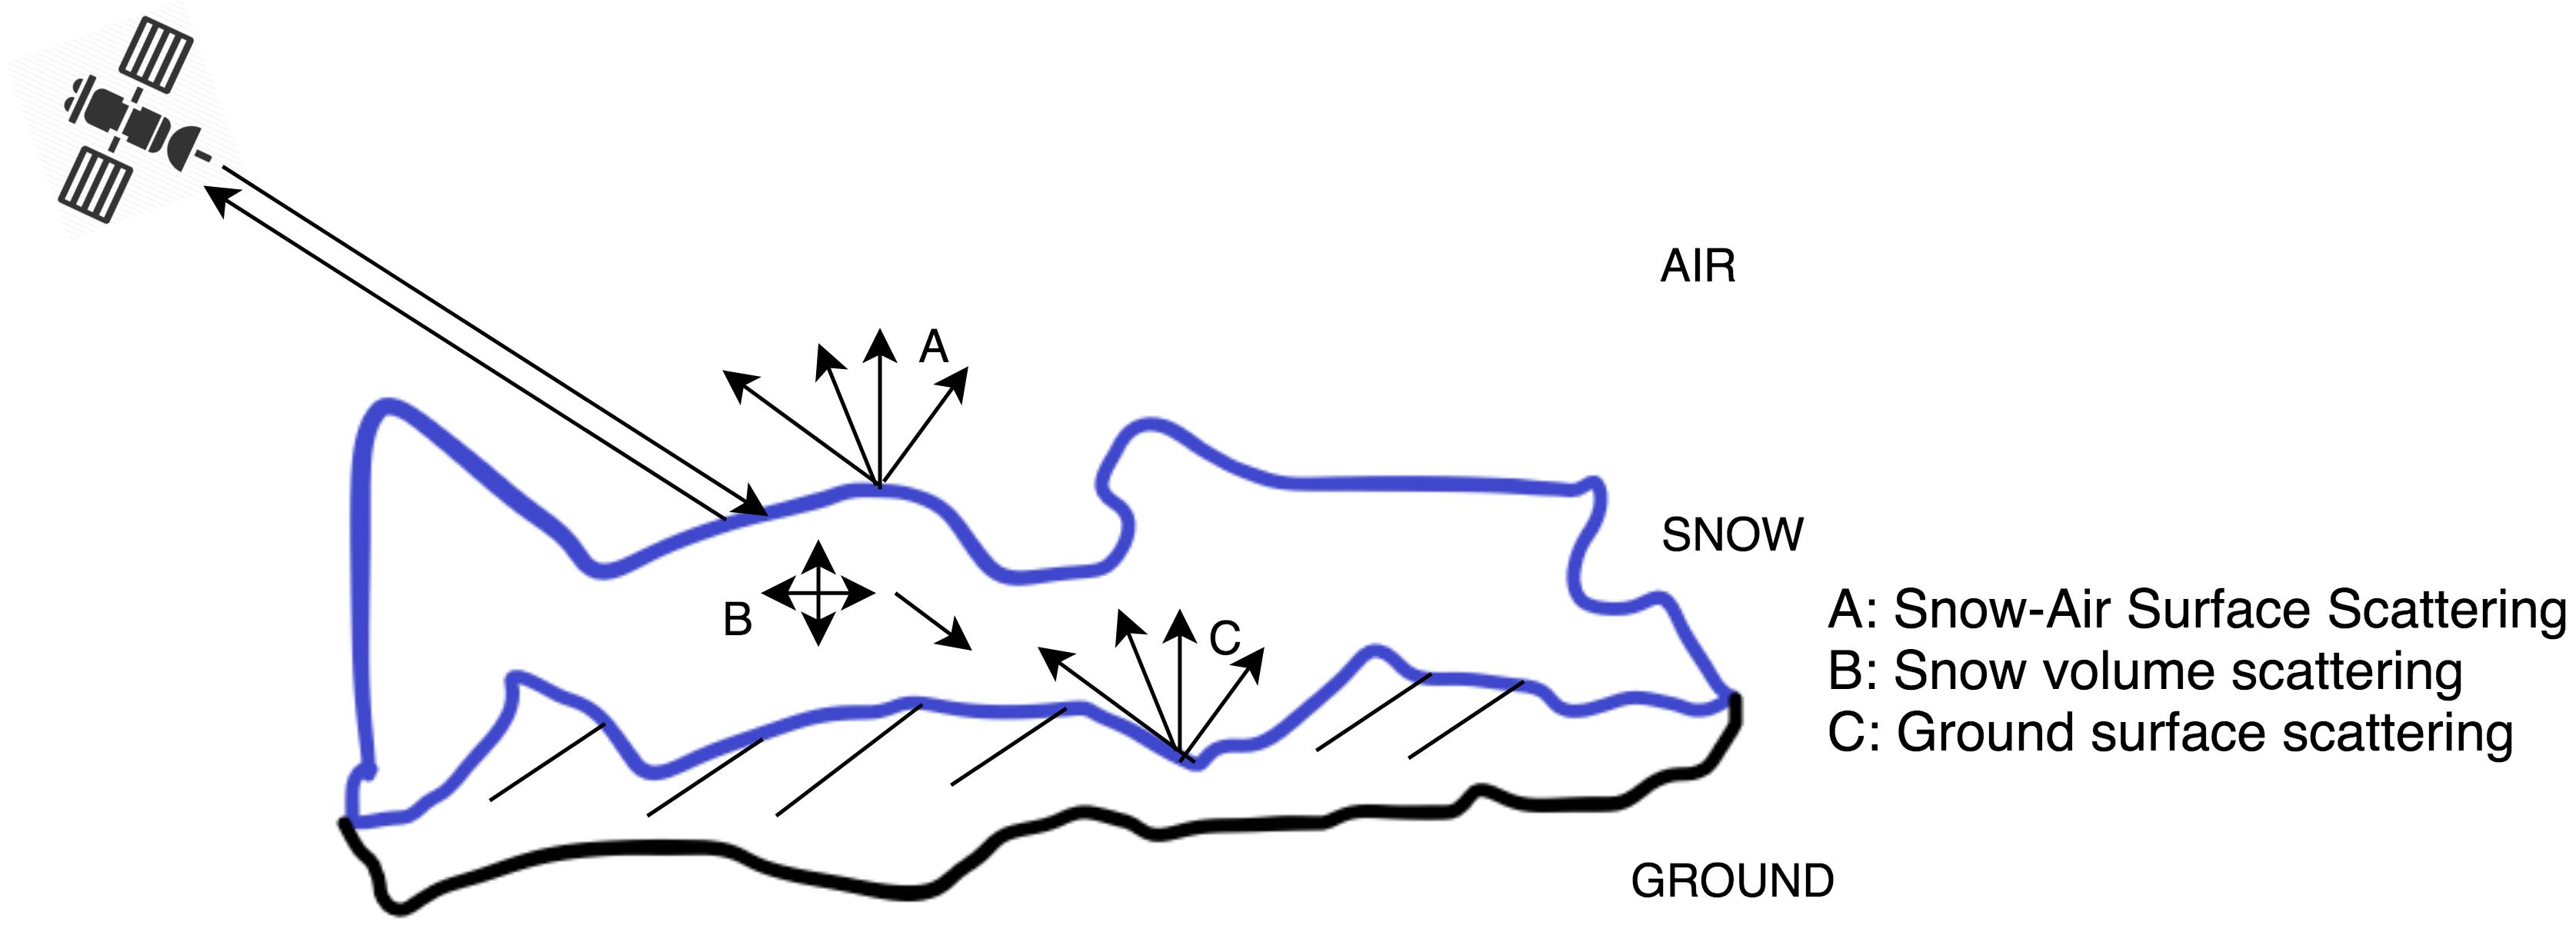
\includegraphics[width=\textwidth]{Figures/Conceptual.png}
    \caption{Conceptual diagram displaying the radar backscattering mechanism in hilly terrains. Adapted from \cite{Thakur2012}.}
    \label{fig:concept}
\end{figure}

A polarimetric SAR system utilises the polarised radar echoes to obtain information about the specific scattering mechanism for a particular target. In essence, by using a coherent analysis which incorporates the phase of different polarimetric channels, it is possible to differentiate various scattering mechanisms \citep{Lee2009}. Nowadays, PolSAR based algorithms that work on the polarimetric backscatter signal have been widely adopted for various snow related applications such as the classification of dry and wet snow, measuring snow wetness and snow density \citep{Singh2017, Snehmani2010, Thakur2012, Thakur2017, Usami2016}. In this context, the roll-invariant entropy-anisotropy-alpha (H-A-$\alpha$) decomposition and Wishart classification have been successfully tested to classify different snow types as well as demarcate snow covered areas \citep{Cloude2010,Lee2009,Singh2014}. A few years back, the use of spaceborne PolSAR for snow height determination had been introduced, wherein the relationship between the copolar phase difference (CPD) and fresh snow depth (FSD) is quantitatively analysed by deriving a theoretical model \citep{Leinss2014}. However, the major challenge in this approach lies in accurately modelling the anisotropic effective permittivity of dry snow which is dependent on the depolarisation factor (calculated by fixing the shape of the ice grain) and ice grains’ volume fraction (measured using snow density).

Interferometric SAR techniques find significant usage in the cryosphere domain and have been used to construct highly accurate digital elevation models (DEMs), measure dry snow depth and SWE in several studies \citep{Guneriussen2001, Lei2016, Leinss2015, Li2017, Liu2017}. The principle of SAR interferometry builds upon measured phase differences between radar images of the same area acquired at different temporal instances (repeat-pass) or different viewing geometries but same epoch (single-pass) \citep{Hanssen2001}. Still, the inherent problems of spatial and temporal decorrelations and atmospheric inhomogeneities are the primary limiting factors in the studies involving InSAR and its variant D-InSAR (Differential InSAR) \citep{Pepe2017}. While spatial decorrelation is caused by large perpendicular baselines \citep{Pepe2017}, the problem of temporal decorrelation arises due to the change in the surface over time \citep{Leinss2018, Leinss2015}. Moreover, the atmospheric noise occurs owing to the variation in the water vapour distribution in the atmosphere \citep{Hanssen2001}. These factors are responsible for inaccurate and low-coherence measurements, thereby leading to a potential decrease in the accuracy of the final results. In cryosphere research, the loss of coherence in InSAR is heavily influenced by the snow humidity, melting, and refreezing and is also susceptible to the variations in both spatial and temporal baselines. Although data assimilation algorithms like 3DVAR (three dimensional variation) and EnKF (Ensemble Kalman Filter) have been applied to the produced outputs of the SD inversion models for minimizing the effect of temporal decorrelation, the applicability and feasibility of such algorithms remains untested on varying data sets and study areas \citep{Liu2017}.

The Pol-InSAR technique works on the coherent combination of both PolSAR and InSAR observations, thereby enabling the interferogram generation in arbitrary transmit and receive channels \citep{Cloude1998, Cloude2005, Cloude2010}. It has been widely used for estimating tree height in forested regions and can be effectively applied to natural or artificial volume scatterers including snow and ice \citep{Hajnsek2009, Kugler2015, Kumar2017, Papathanassiou2001}. In essence, the identification of different scattering processes (PolSAR) and the vertical profile sensitivity (InSAR) are unique to this technique. Therefore, the applicability of Pol-InSAR based SD retrieval could prove its potential in case of the standing snow depth (SSD) \citep{Negi2009, Thakur2012, Thakur2017}.

The prime focus of this research is to estimate the FSD and SSD using PolSAR and Pol-InSAR respectively. In addition, the corresponding fresh SWE (FSWE) and standing SWE (SSWE) are to be determined, for which the respective snow densities need to be known. Essentially, the study involves sensitivity analysis of the various model parameters along with the identification of the different uncertainty sources present in the chosen geographical area. 

This manuscript is compartmentalised into five sections each consisting of several subsections. It starts with an introductory discussion in section \ref{sec:Intro}. Thereafter, the study area and the datasets including the required  software are specified in section \ref{sec:study}. From section \ref{sec:method} onwards the methodology and results are discussed. Finally, the relevant conclusions and recommendations are put forward in section \ref{sec:conc}.

\section{Study Area, Datasets, and Software}
\label{sec:study}

\subsection{Chosen Study Area}
\subsubsection{Geographical Situation}

The Beas river watershed near Manali, India is part of the north-western Himalayas. Naturally, steep slopes and dense forests are prominent in this region. The elevation typically varies from nearly 2500 m to more than 5000 m in some places as observed in the reference ALOS PALSAR DEM (Figure \ref{fig:overview}). 

\begin{figure}[htb]
    \centering
    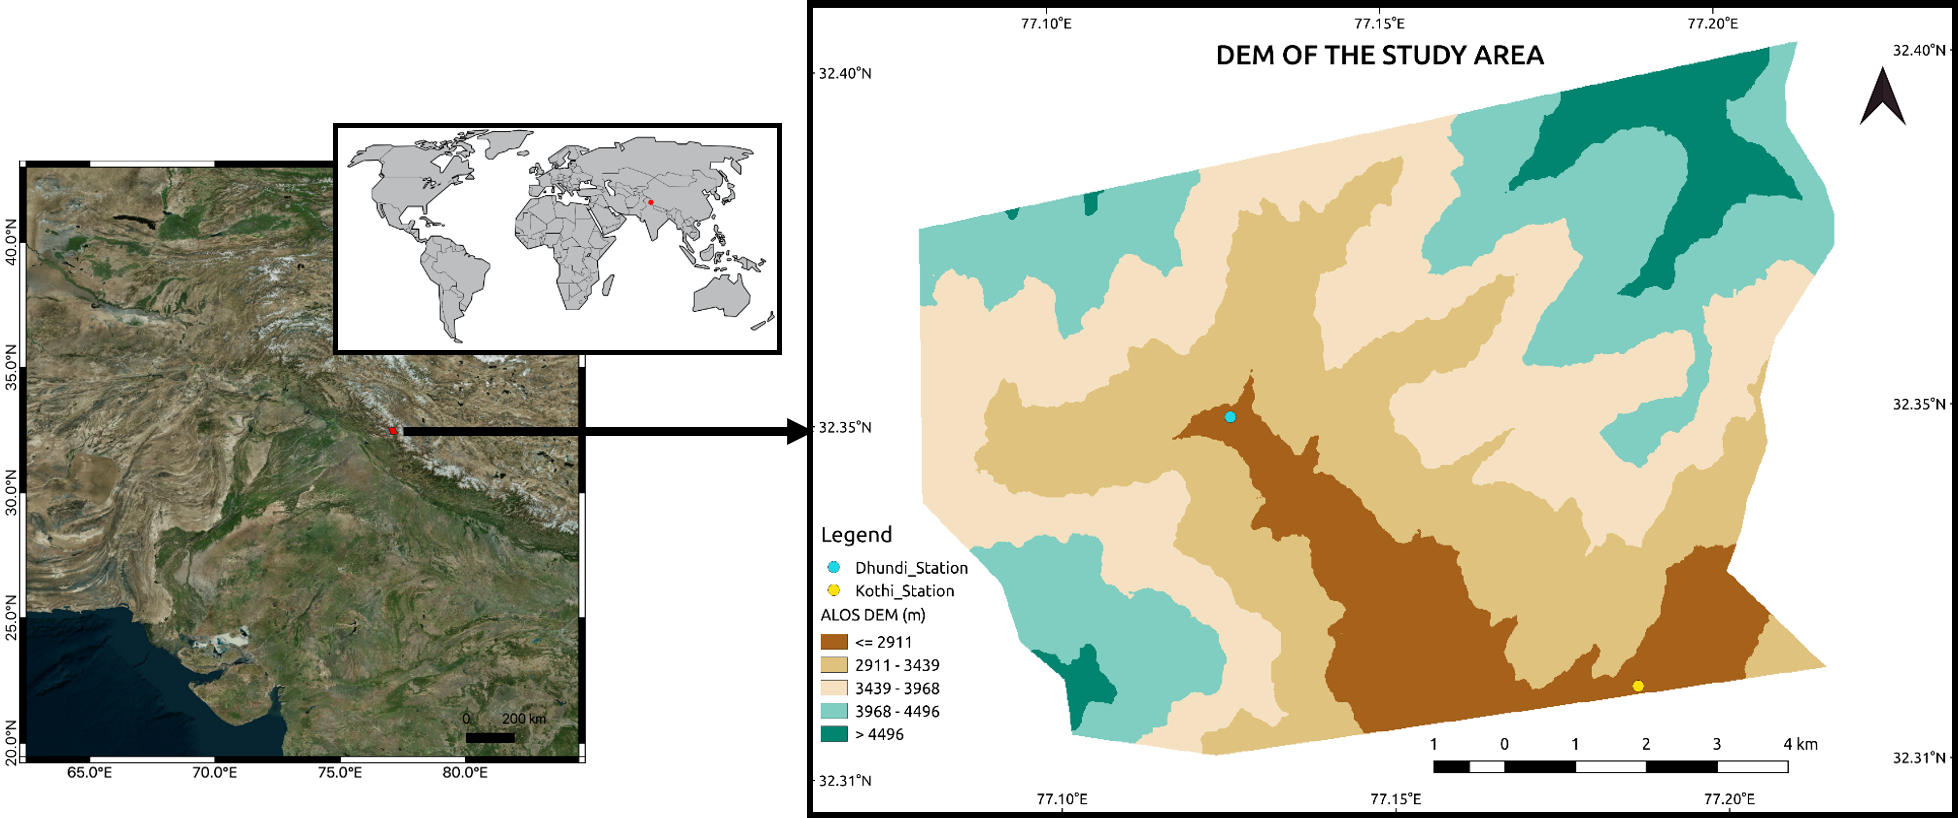
\includegraphics[width=\textwidth]{Figures/Overview.png}
    \caption{Overview map of the study area showing the ALOS PALSAR DEM. The original DEM of 12.5 m spatial resolution (generated in 2011) has been resampled to 3 m using bilinear interpolation \citep{Wu2008} to match the high resolution SAR data. Moreover, the vertical resolution as per the product specification is 5 m.}
    \label{fig:overview}
\end{figure}

In this work, a small region ($\sim$ 96 km\textsuperscript{2}) of the Beas basin is chosen which starts a few kilometres uphill from Dhundi up to Kothi (shown in Figure \ref{fig:overview}). These areas receive substantial seasonal snowfall which begins in December and lasts till late March. However, the cold, dry season usually commences from late September or early October. The coldest period is in January during which the temperatures reach a daily minimum of -15$^\circ$C on an average. The summers are mild to occasionally warm with June being the hottest month (mean and maximum temperatures of 20$^\circ$C and 30$^\circ$C respectively are common). Apart from this, significant rainfall occurs between late June and September (monsoon season) with August receiving the maximum precipitation \citep{Majumdar2019, Thakur2012}.

\subsubsection{Field Visit}

Intensive fieldwork had been conducted from October 14-21, 2018 in the Dhundi and Kothi areas where several Differential Global Positioning System (DGPS) measurements were acquired using the Leica Viva GS 10 \citep{LeicaGeosystemsAG2012} with adequate horizontal positional accuracies ($\sim$7 cm) \citep{Majumdar2019}. Due to the complex terrains, most of the DGPS readings had been obtained through the kinematic mode \citep{Luo2014}. However, in some of the convenient places such as the Dhundi base station and near the Kothi Automatic Weather Station (AWS), the static mode was used \citep{LeicaGeosystemsAG2012}. Eventually, elevation information from these DGPS points have been compared with the ALOS PALSAR DEM, the details of which are provided in section \ref{sec:res}. Furthermore, the manual snow readings from 2014-2018 (snow depth, density, weather profile and other relevant data) which are maintained by the security personnel daily at Dhundi had been pagewise photographed using a smartphone camera. In order to properly understand and visualise the characteristics of the study area, selected field photographs and their brief description are shown from figures \ref{subfig:gps}-\ref{subfig:stations}.

\begin{figure}[!t]
    \centering
    \begin{subfigure}[t]{0.49\textwidth}
        \raisebox{-\height}{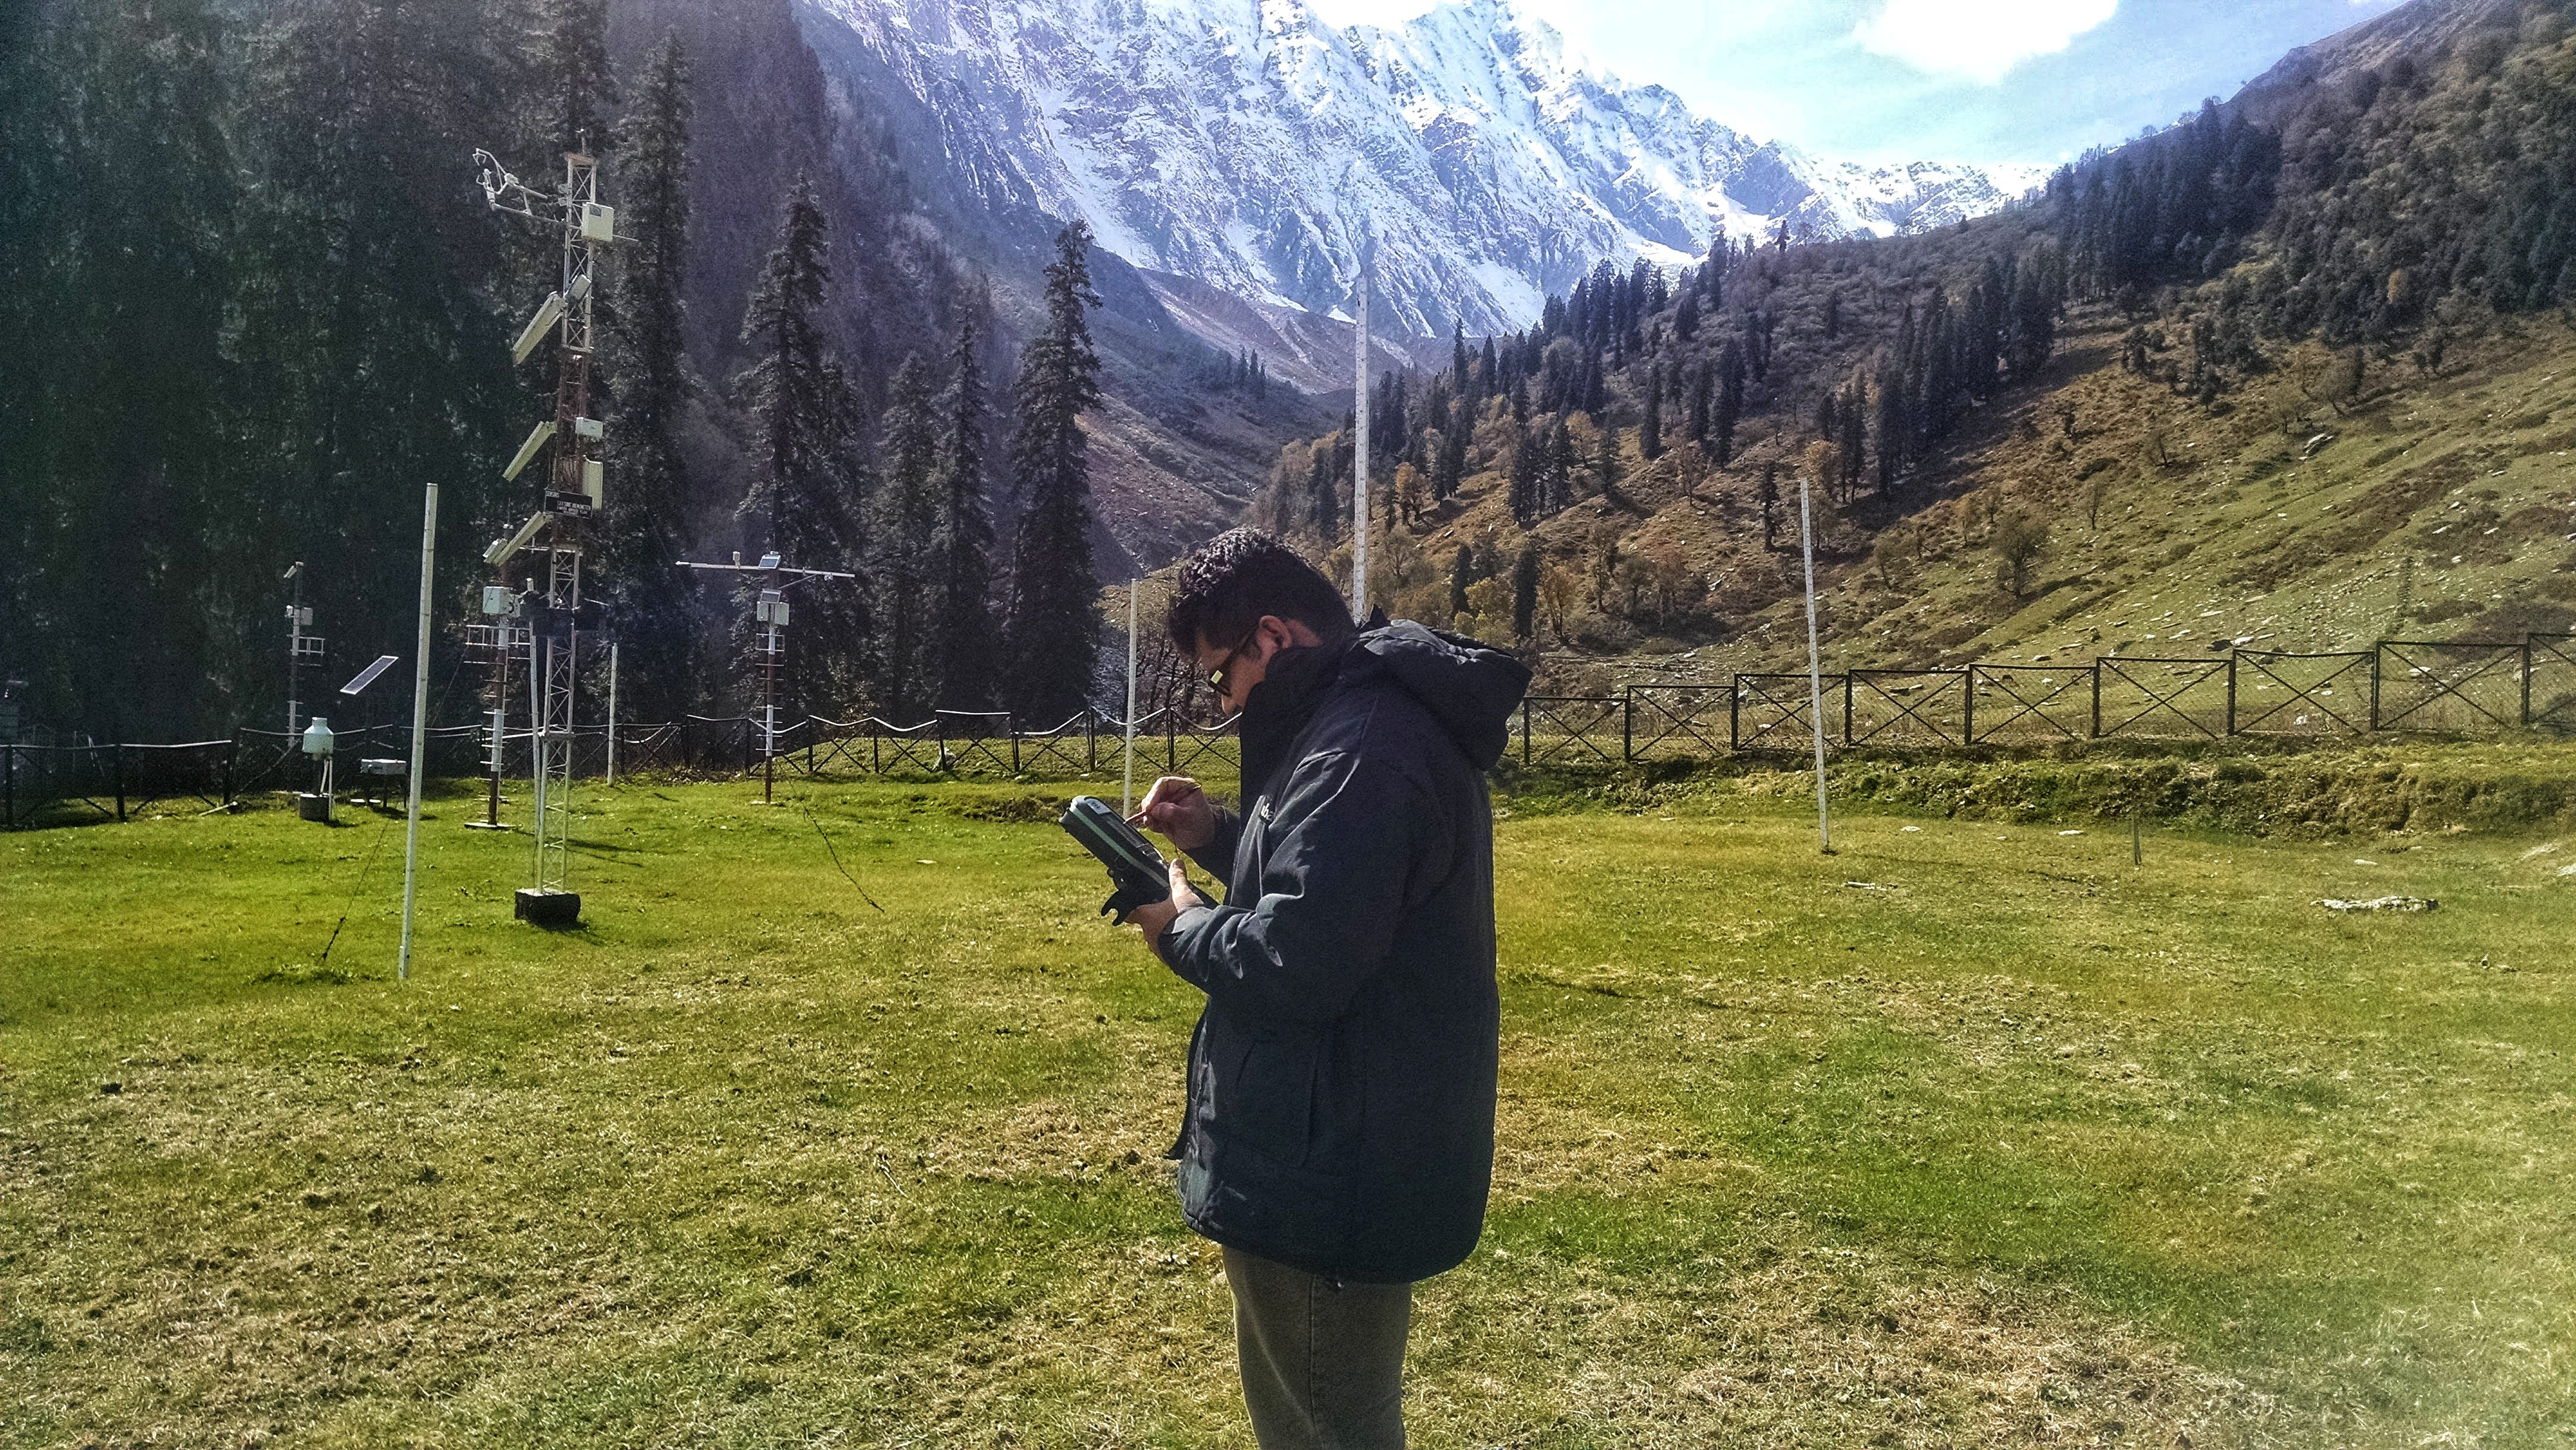
\includegraphics[width=\textwidth]{Figures/Field/me_gps.jpg}}
        \caption{DGPS positional accuracy checking}
        \label{subfig:gps}
    \end{subfigure}
    \hfill
    \begin{subfigure}[t]{0.49\textwidth}
        \raisebox{-\height}{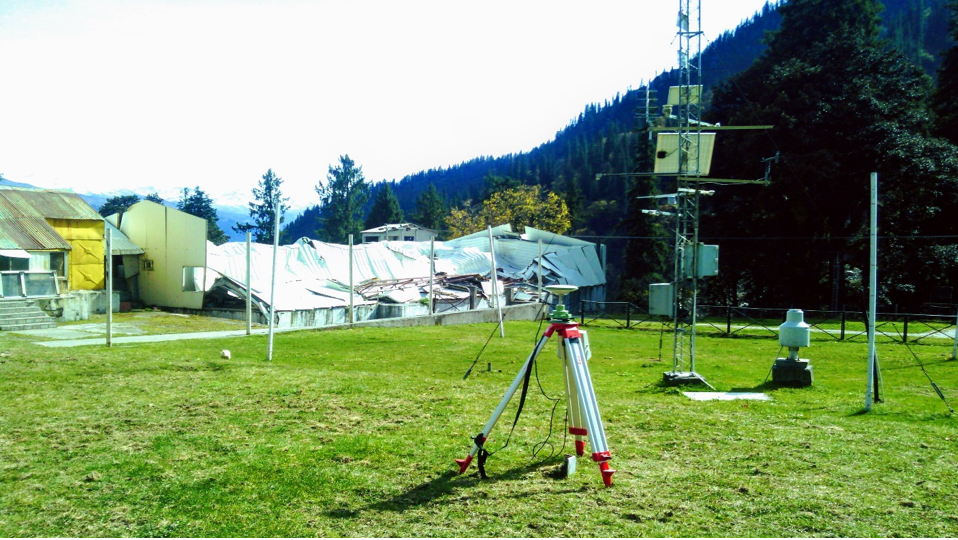
\includegraphics[width=\textwidth]{Figures/Field/base.png}}
        \caption{Leica DGPS base}
        \label{subfig:base}
    \end{subfigure}
    %%%%%%%%%%%%%%%%%%%%%%%%%%%%%%%%%%%%second row
    \begin{subfigure}[t]{0.49\textwidth}
        \raisebox{-\height}{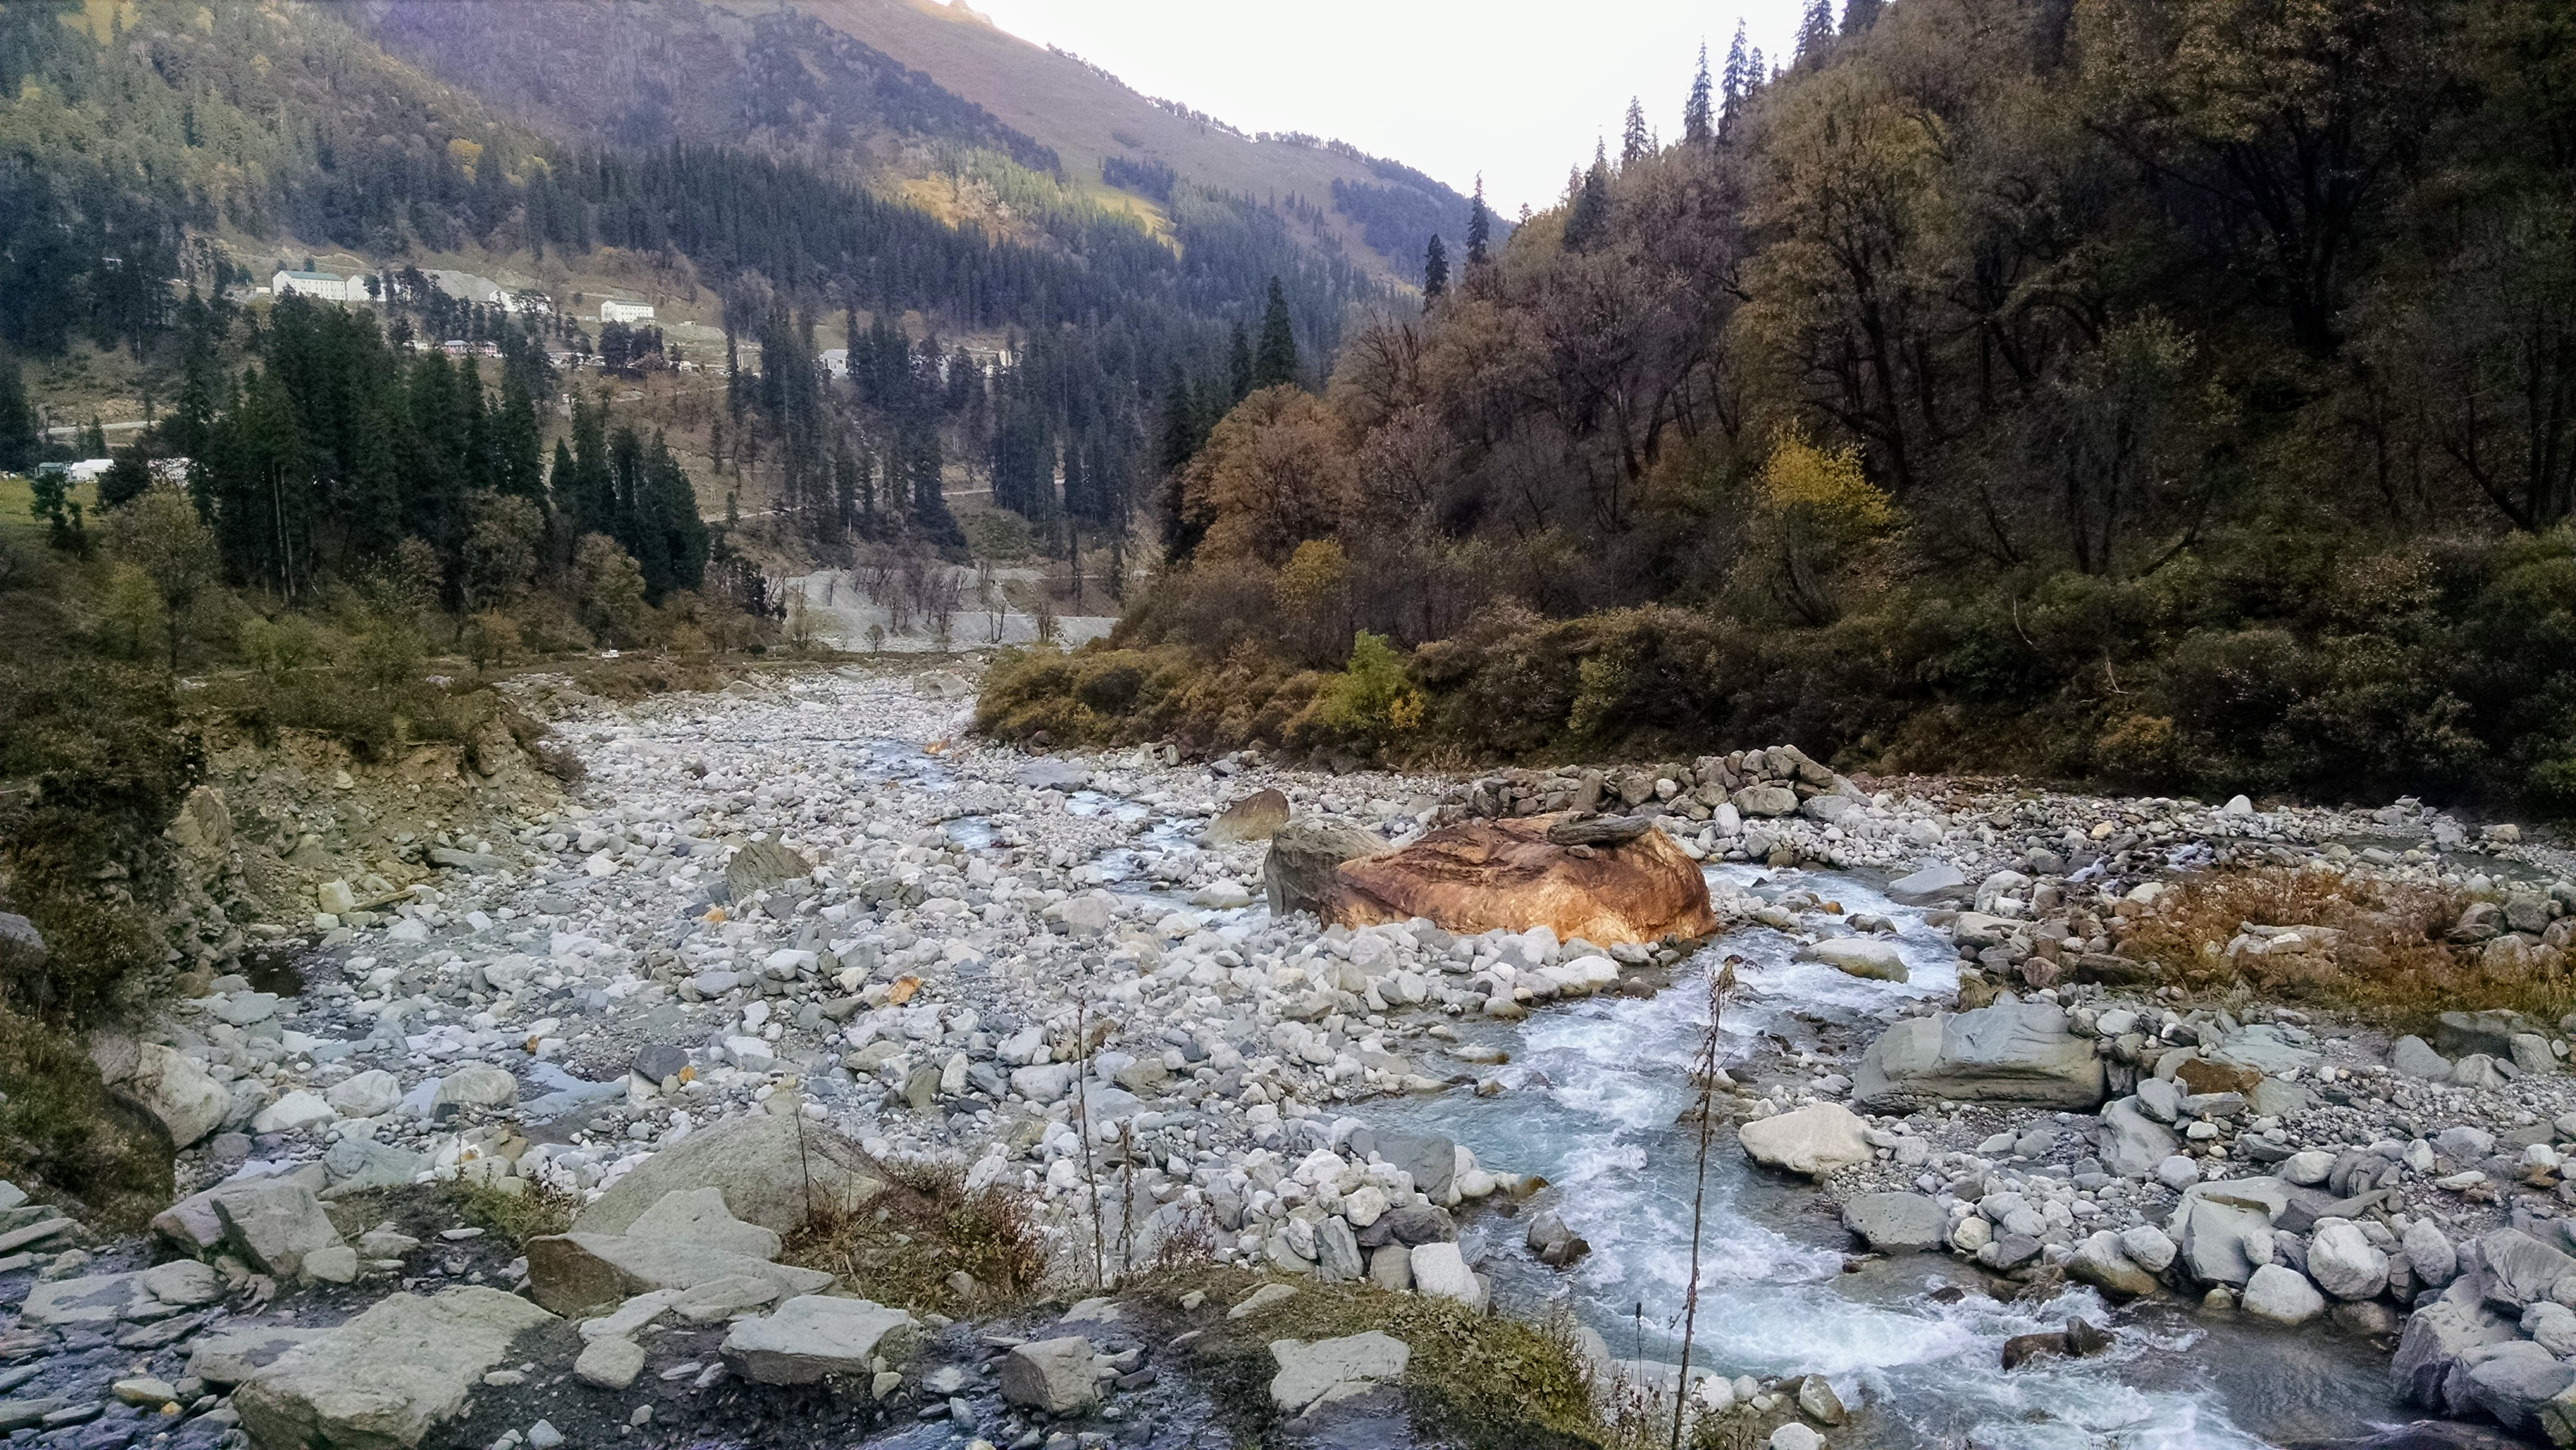
\includegraphics[width=\textwidth]{Figures/Field/beas.jpg}}
        \caption{Beas river}
        \label{subfig:beas}
    \end{subfigure}
    \hfill
    \begin{subfigure}[t]{0.49\textwidth}
        \raisebox{-\height}{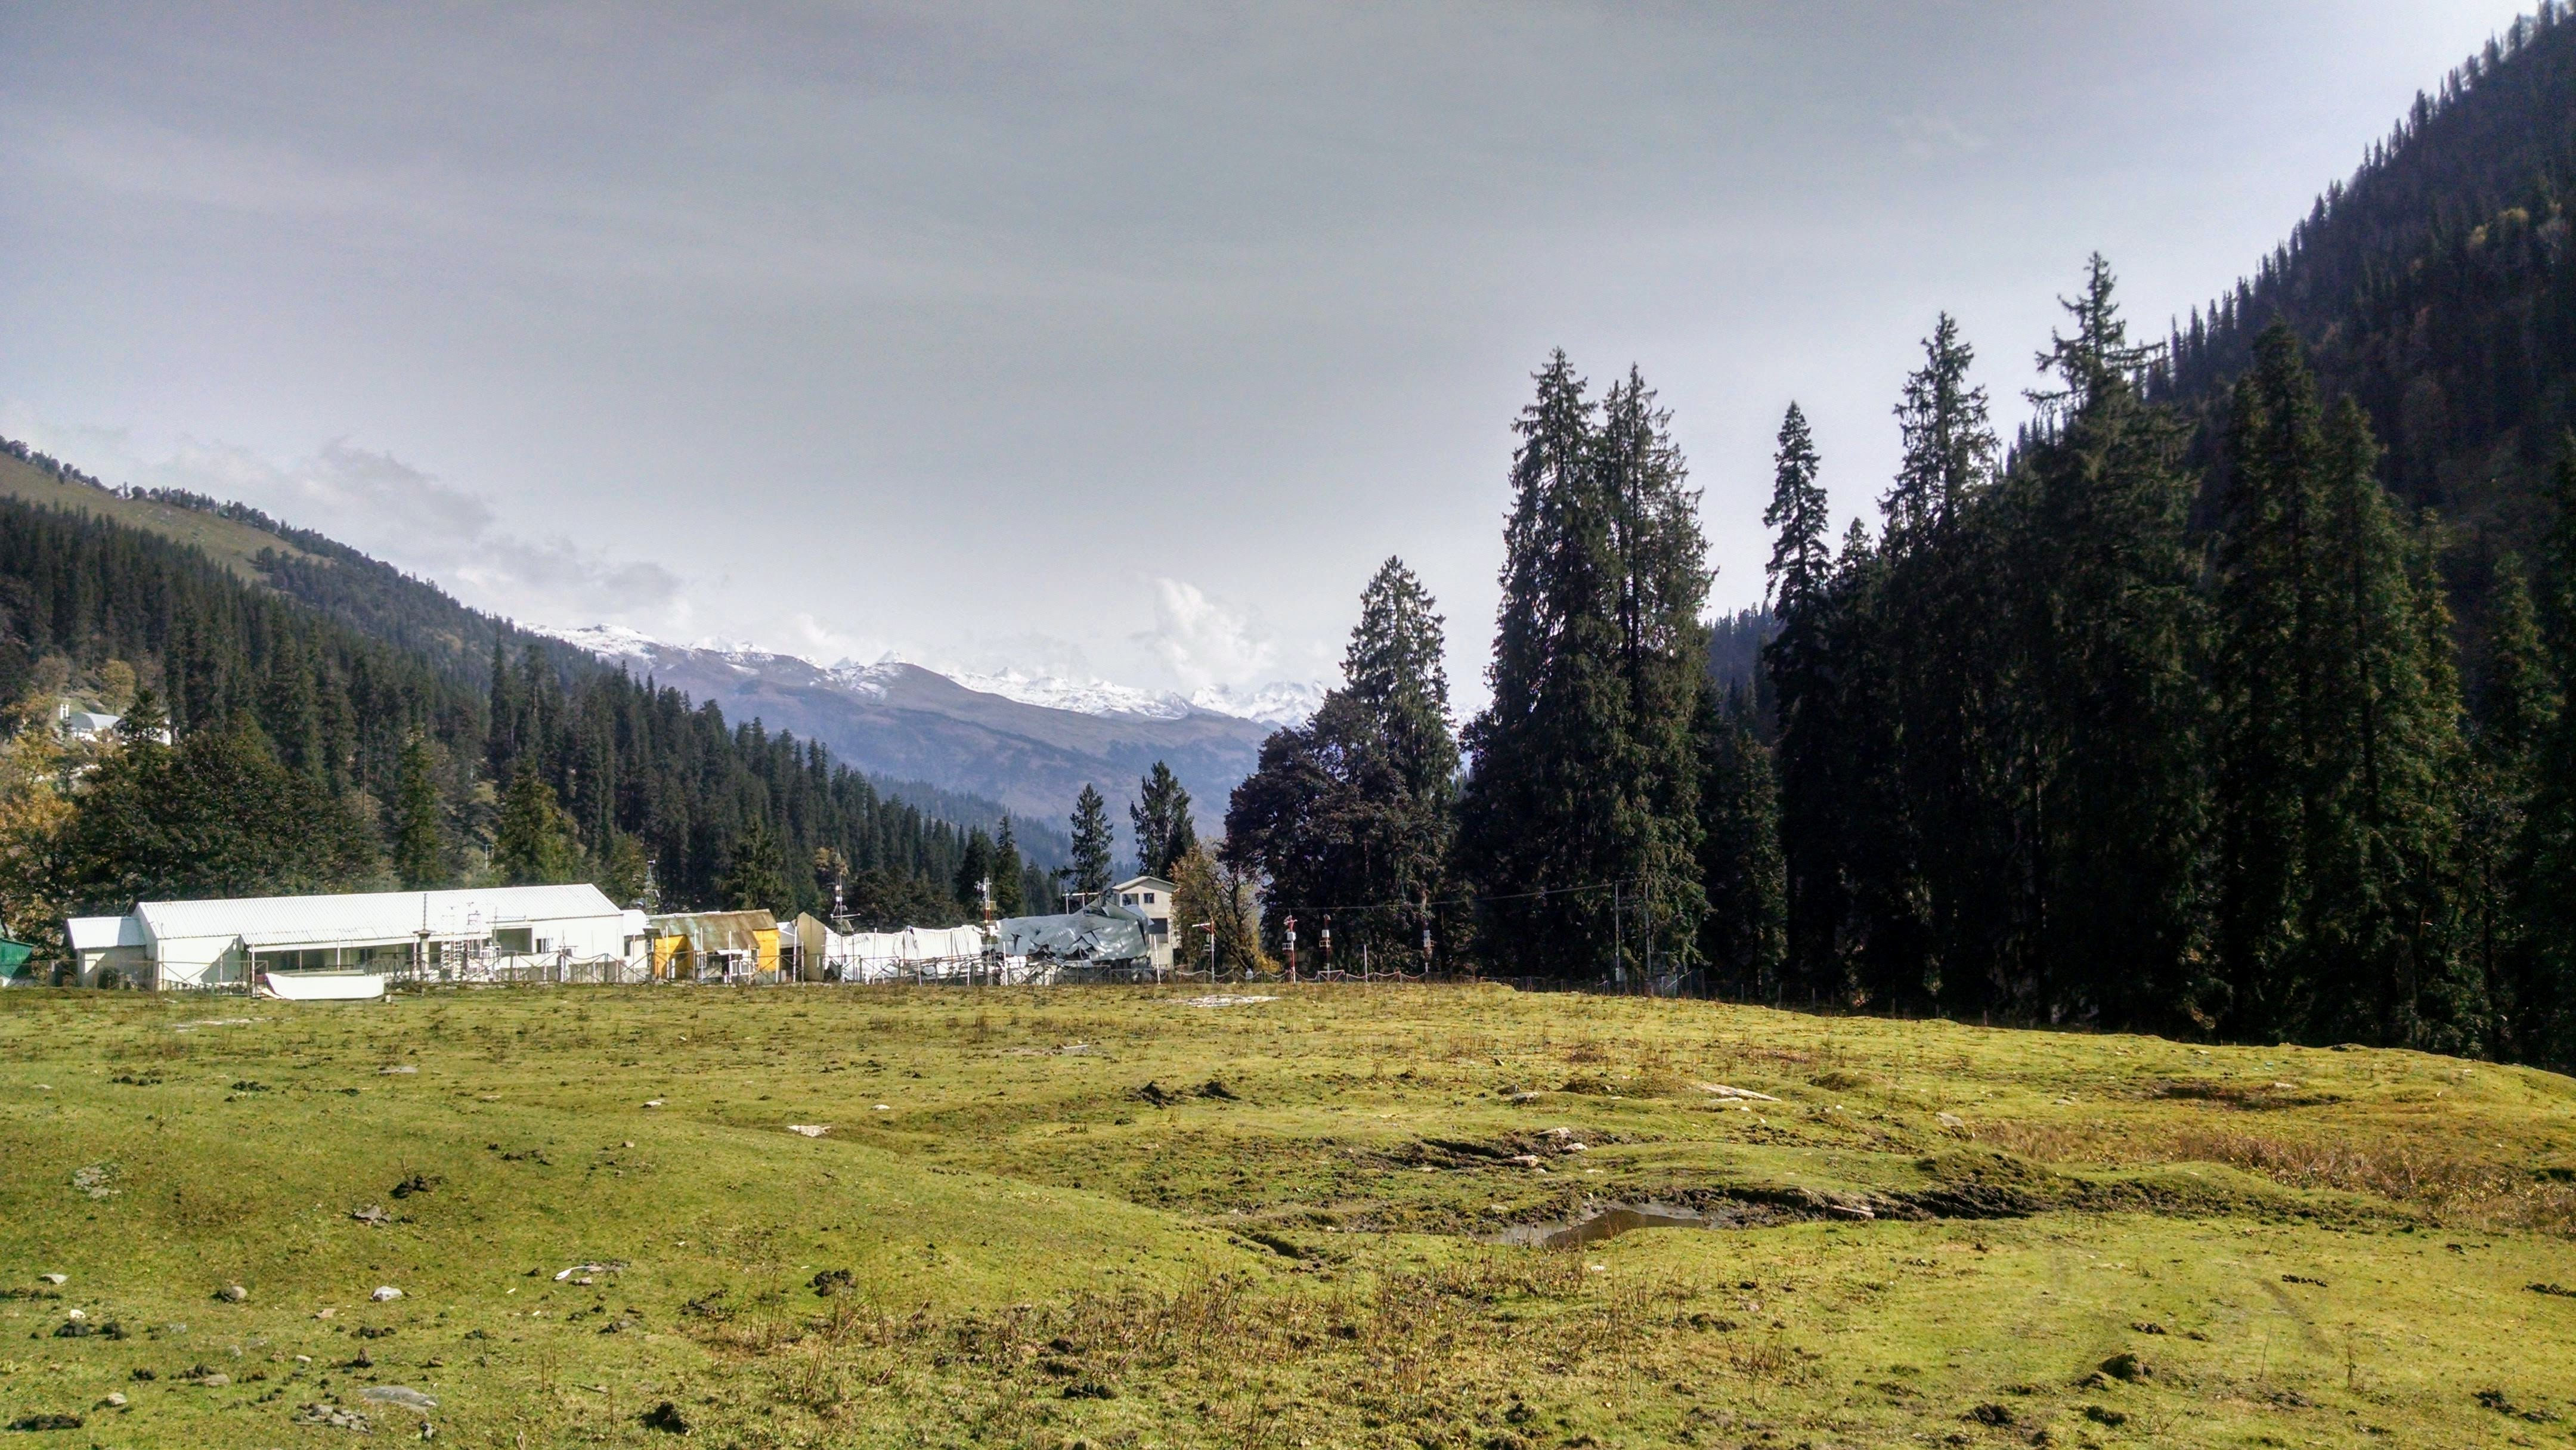
\includegraphics[width=\textwidth]{Figures/Field/landscape.jpg}}
        \caption{Landscape and human settlements}
        \label{subfig:landscape}
    \end{subfigure}
    %%%%%%%%%%%%%%%%%%%%%%%%%%%%%%%%%%%third row
    \begin{subfigure}[t]{0.49\textwidth}
        \raisebox{-\height}{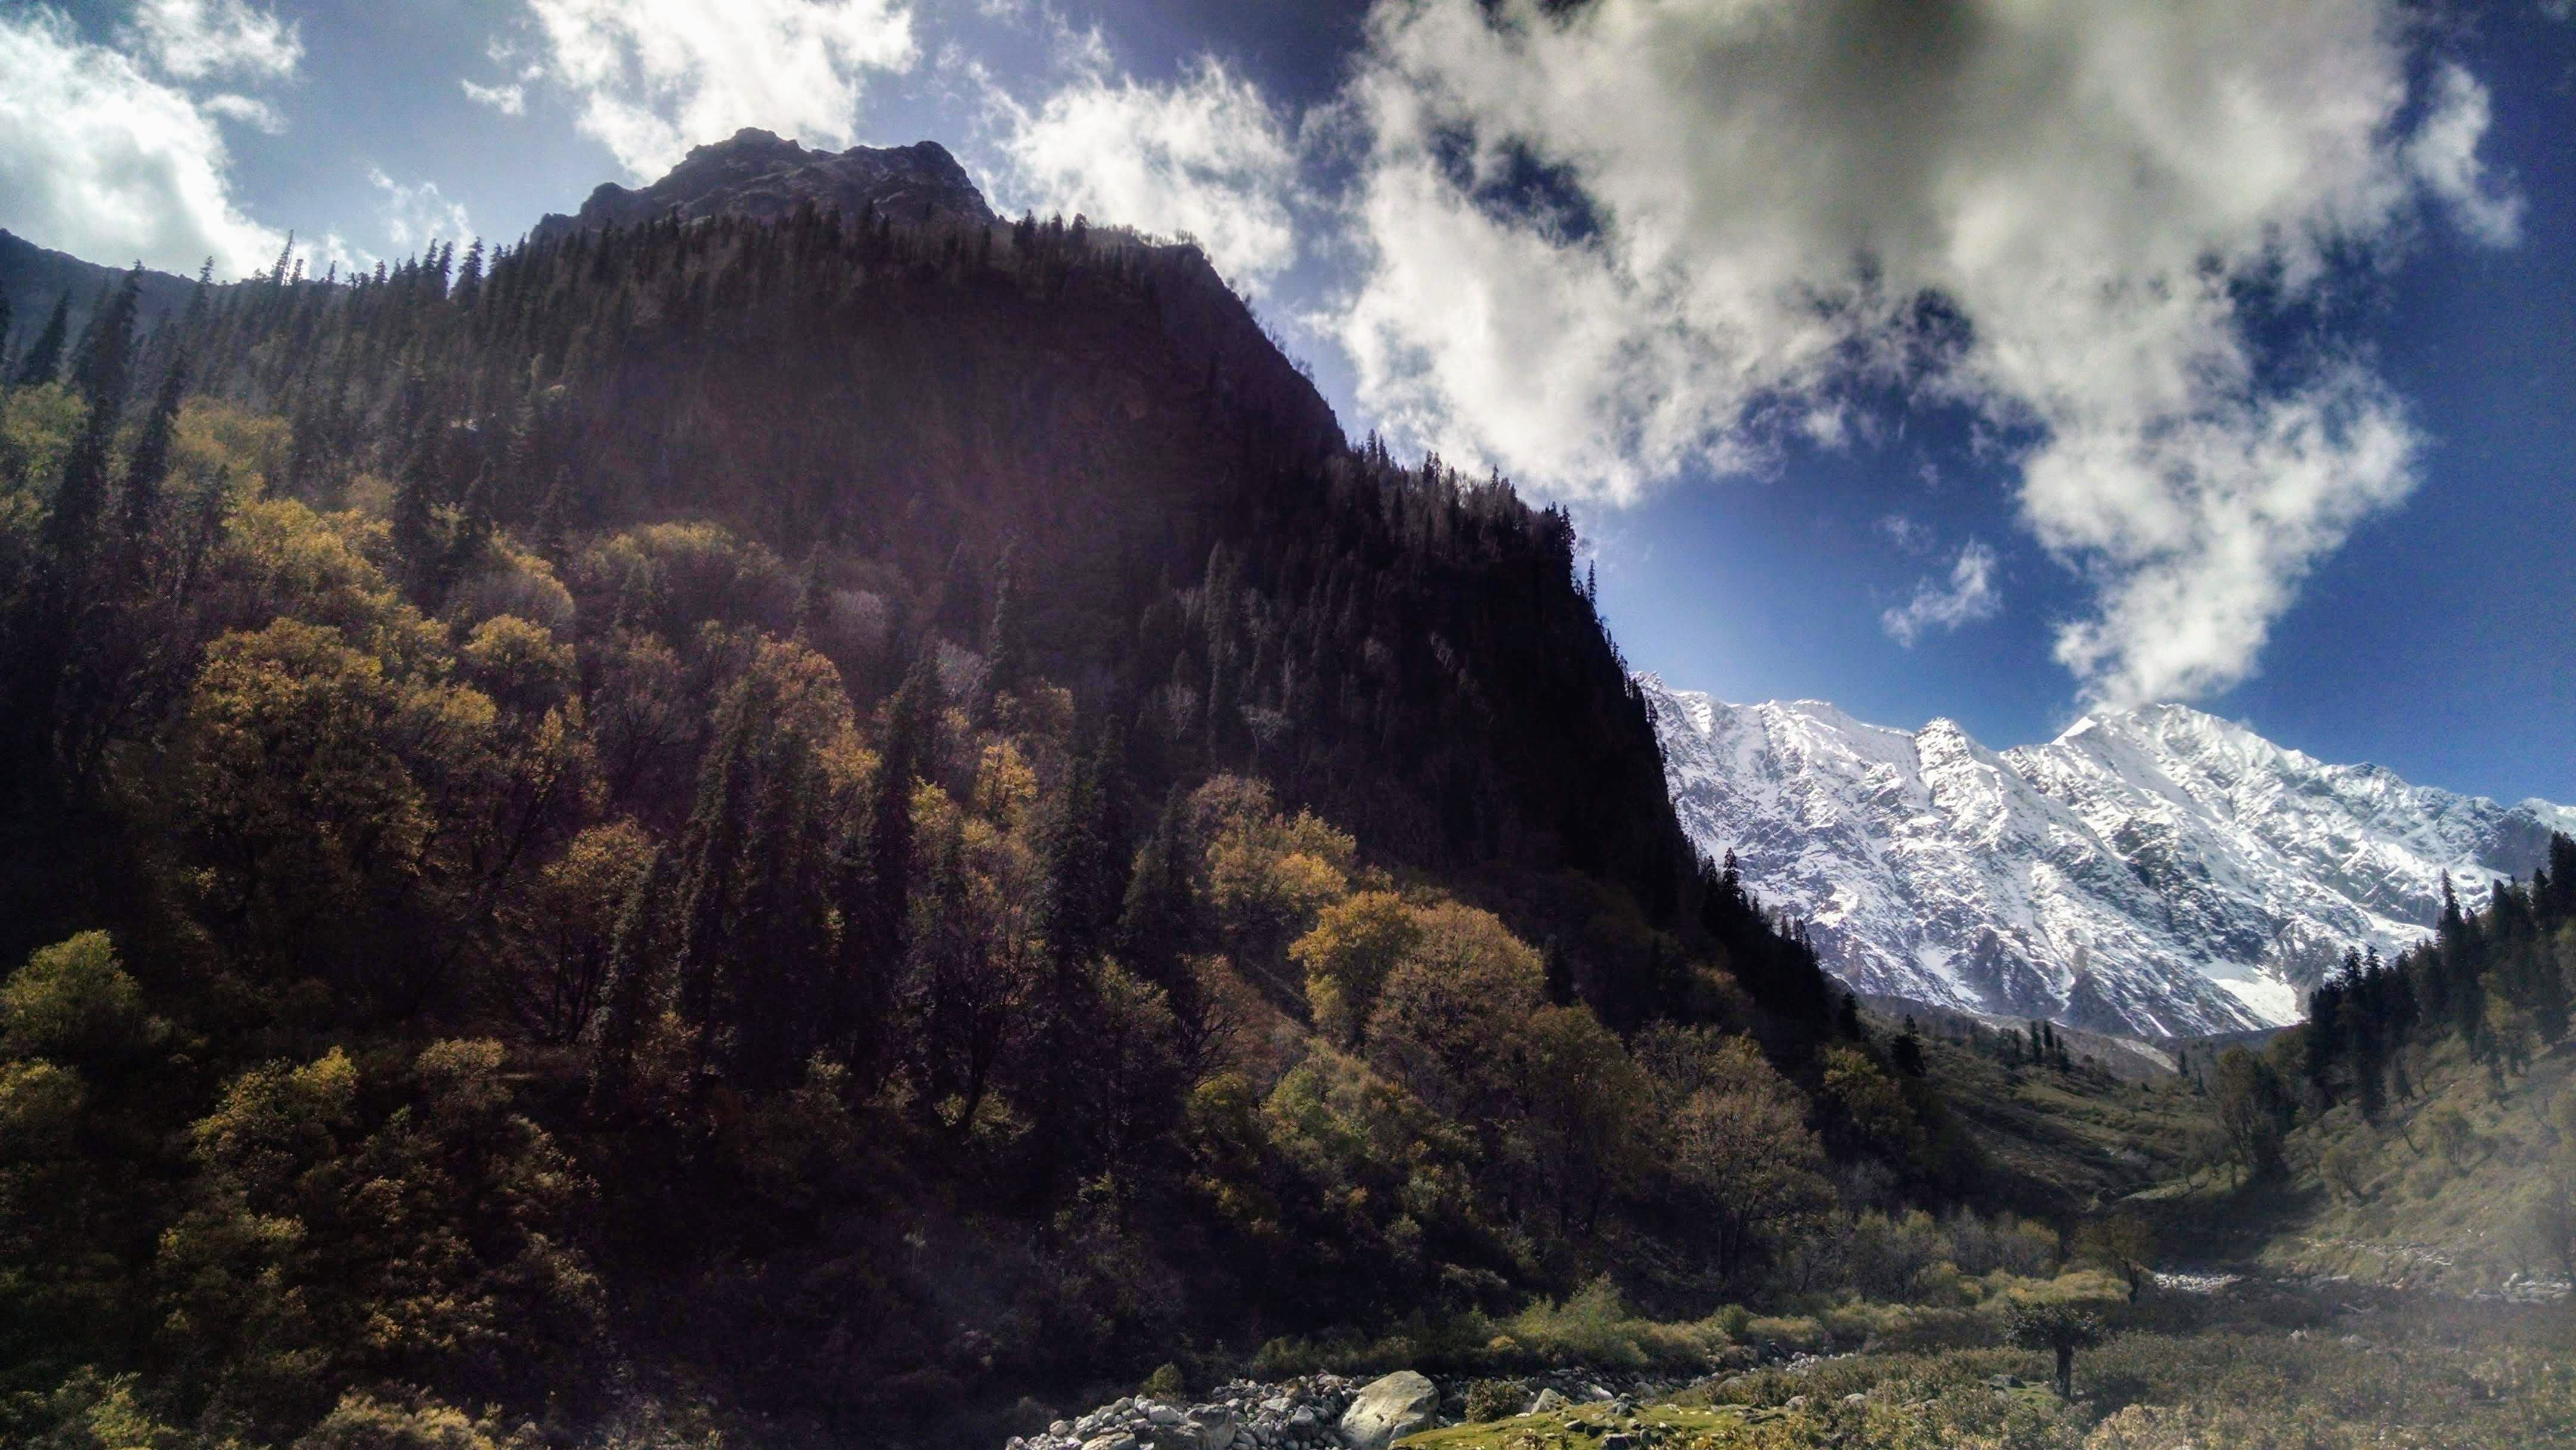
\includegraphics[width=\textwidth]{Figures/Field/mountain.jpeg}}
        \caption{Mountains and forests}
        \label{subfig:mountain}
    \end{subfigure}
    \hfill
    \begin{subfigure}[t]{0.49\textwidth}
        \raisebox{-\height}{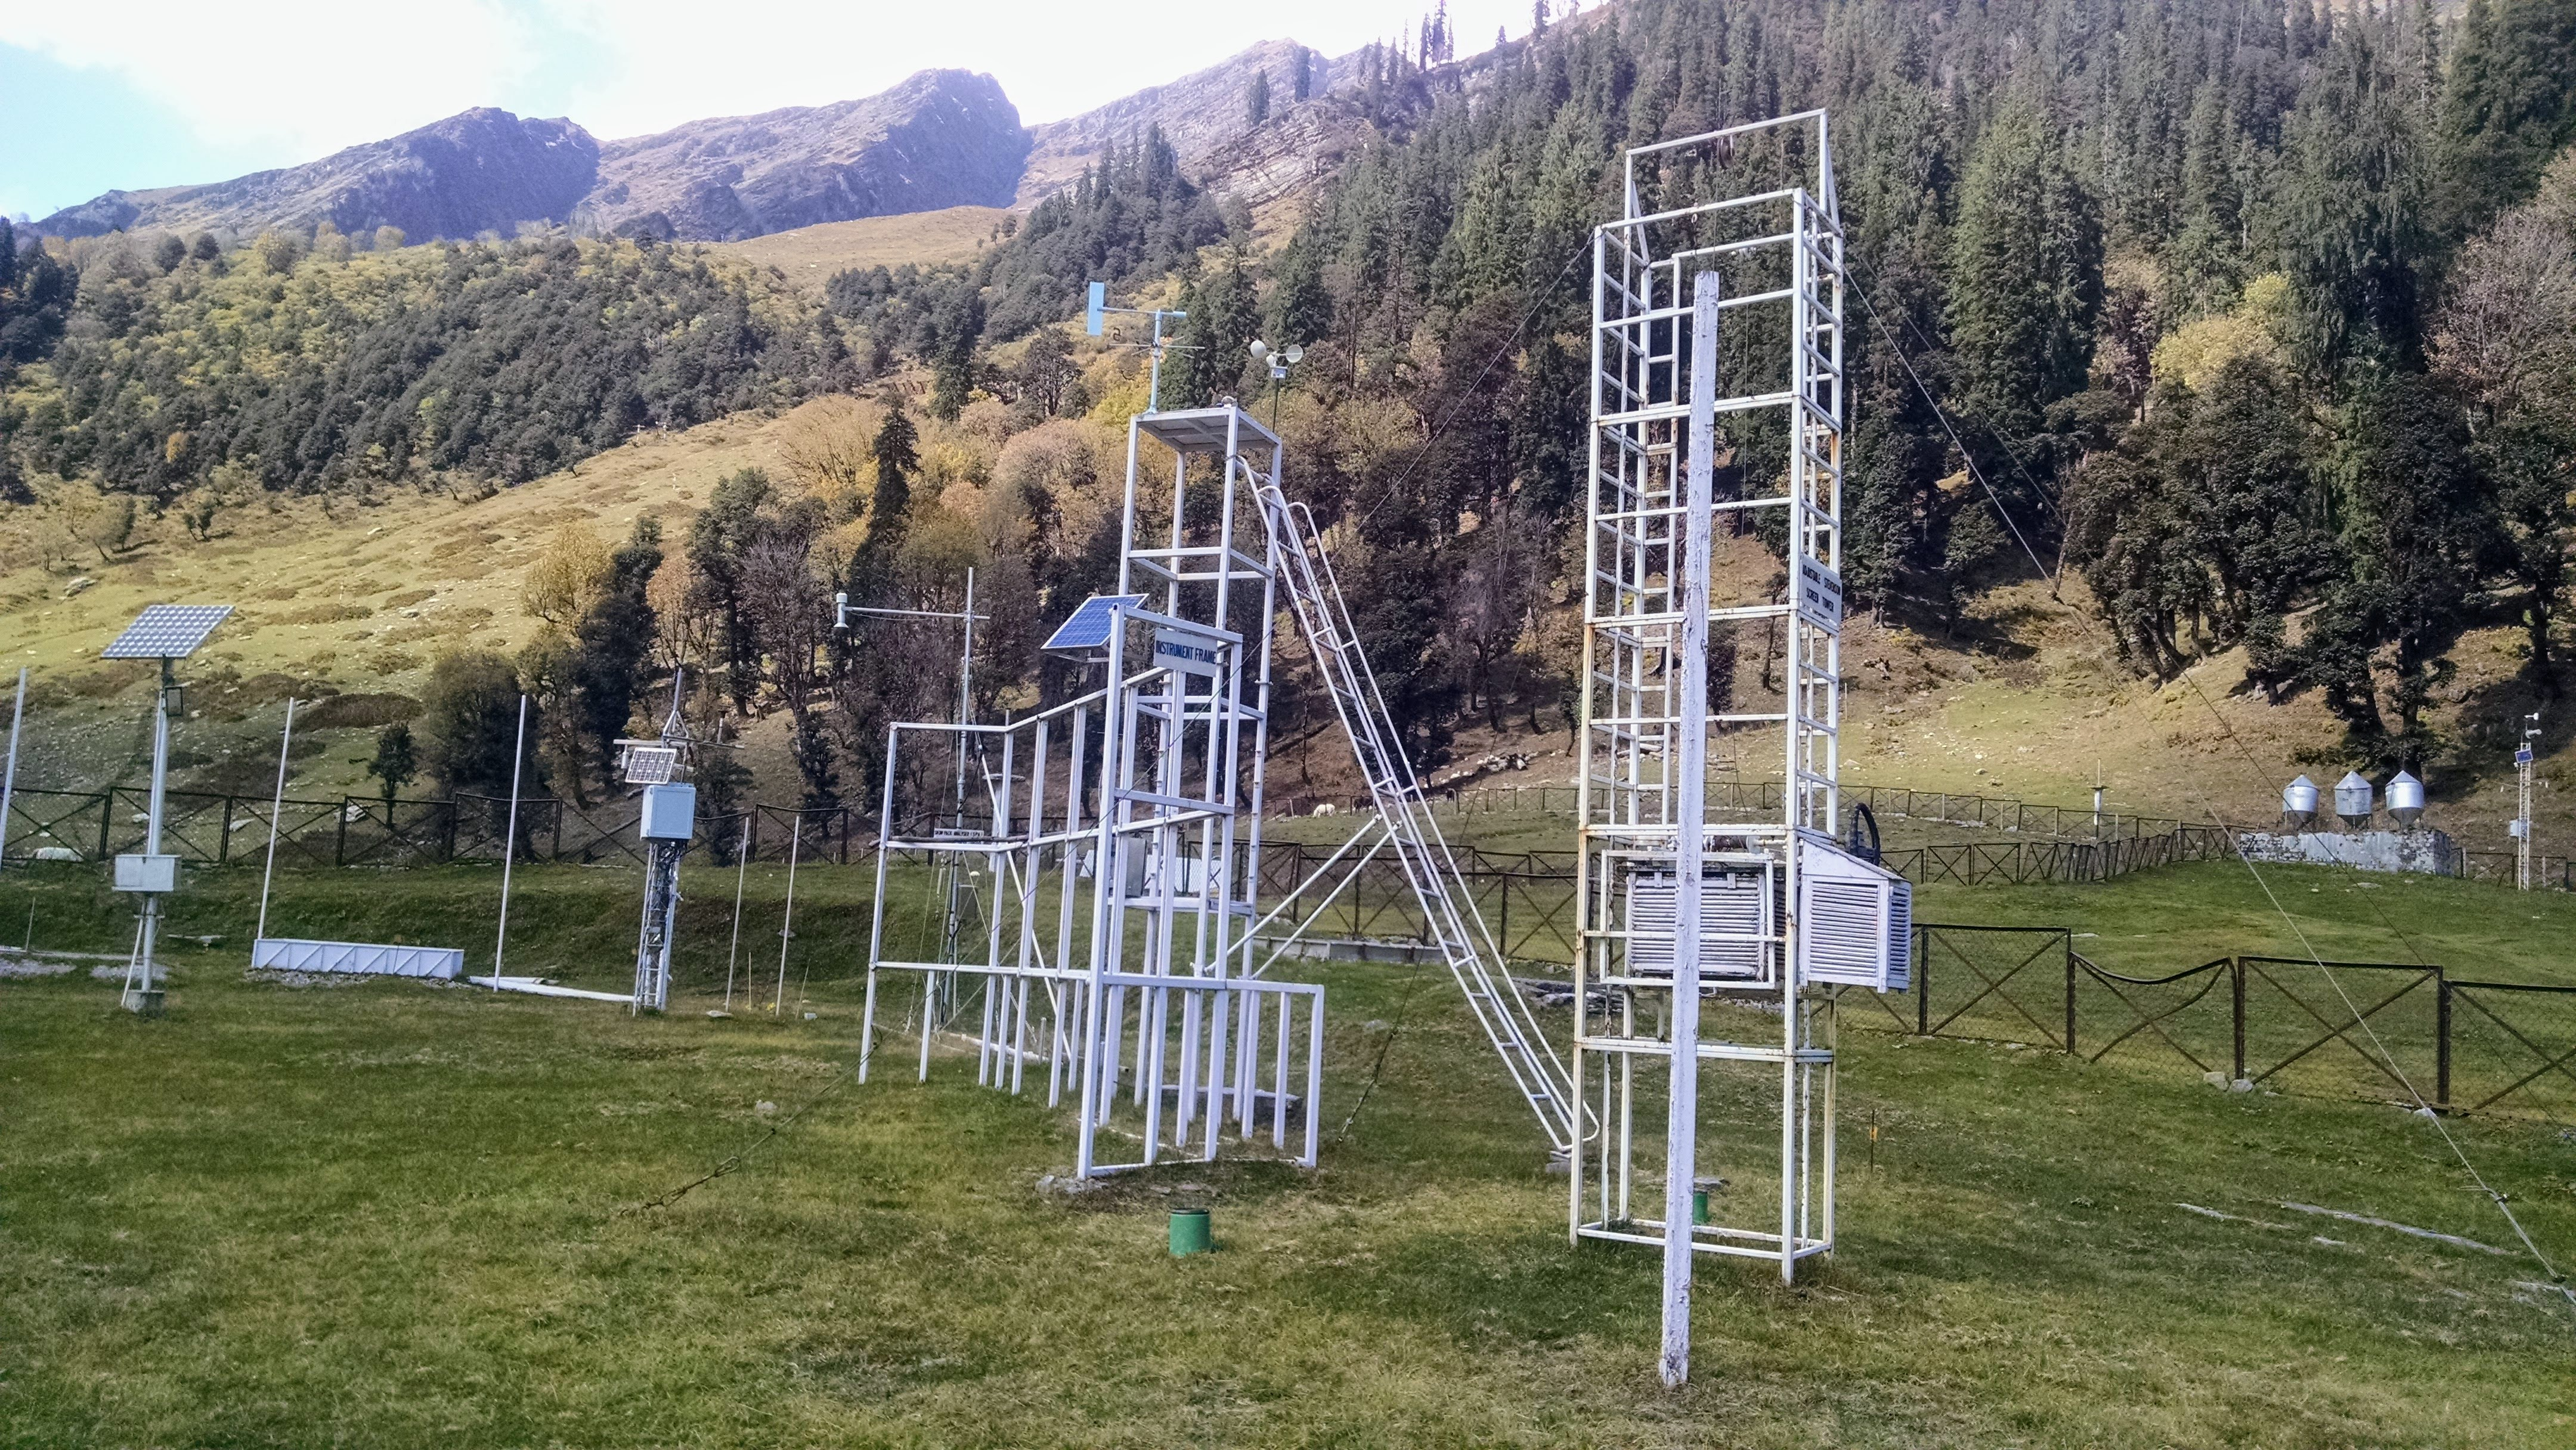
\includegraphics[width=\textwidth]{Figures/Field/stations.jpg}}
        \caption{Weather instruments}
        \label{subfig:stations}
    \end{subfigure}
    \caption{Dhundi field photographs showing the varying topographic features present in the surrounding area.}
    \label{fig:field}
\end{figure}

\subsection{Datasets Used}

Overall twelve Coregistered Single look Slant range Complex (CoSSC) TerraSAR-X (TSX)/TanDEM-X (TDX) bistatic X-band SAR images acquired between December 2015 and August 2017 in stripmap (SM) mode are available over this study area \citep{Balss2012}. In total, there are six Quad-pol data pairs, from which the descending orbital pass acquisition at 00:53 hrs Universal Time Coordinated (UTC), January 8, 2016, has been selected considering the occurrence of fresh snowfall before, during and after the satellite flyby. Moreover, the perpendicular baseline ($B_\bot$) and ambiguity height ($h_{2\pi}$) for this data are 96.34 m and 63.18 m respectively. 

Additionally, the in-situ snow physical parameters’ data (standing and fresh snow depths, snow density) along with the relevant weather data had been transferred to a PostgreSQL database (DB) \citep{PostgreSQL2019} from the photographs of the manual recordings through spreadsheets. Apart from this, the high frequency data (two-minute interval measurements) obtained from the snowpack analyser (SPA) device (installed at Dhundi) had been downloaded and were added to the database as a separate table. Accordingly, the SSDs at 06:22 hrs (00:52 hrs UTC) Indian Standard Time (IST) on January 7, 2016, and 06:22 hrs January 8, 2016 morning were 36.2 cm and 54.9 cm respectively signifying a heavy fresh snowfall event of 18.7 cm within 24 hrs. The manual recordings also showed an FSD of 18 cm on January 8, 2016 morning though the exact measurement time is unspecified in the record book. Apart from this, a forest mask used in the earlier studies of this area \citep{Thakur2012, Thakur2017} has been obtained from the Water
Resources Department (WRD), Indian Institute of Remote Sensing (IIRS).

\subsection{Software}

The Sentinel Application Platform (SNAP) 6.0.5 \citep{ESA2018} has been used for basic SAR processing. In addition, the FSD and SSD inversion models have been implemented using Python 3 wherein PyCharm Community Edition 2018.1 \citep{JetBrains2018} was used as the Integrated Development Environment (IDE). Moreover, the final SD and SWE maps have been prepared using QGIS 2.18 \citep{QGIS2016}. Furthermore, some of the computationally intensive tasks have been carried out using the High-Performance Computing (HPC) infrastructure installed at IIRS.

\section{Methodology}
\label{sec:method}

This section deals with the methodological framework which has been followed to generate the SD and SWE results. In order to briefly put the overall workflow, a flowchart is shown in Figure \ref{fig:method_overview} which highlights the main process blocks. Here, the preprocessing steps are discussed in section \ref{ssec:pre}. Moreover, the PolSAR CPD and Pol-InSAR based approaches used for the FSD and SSD estimation respectively are individually addressed in sections \ref{ssec:fsd} and \ref{ssec:ssd}. Finally, the uncertainty assessment, validation and sensitivity tasks are described in section \ref{ssec:vus}.

\begin{figure}[htb]
    \centering
    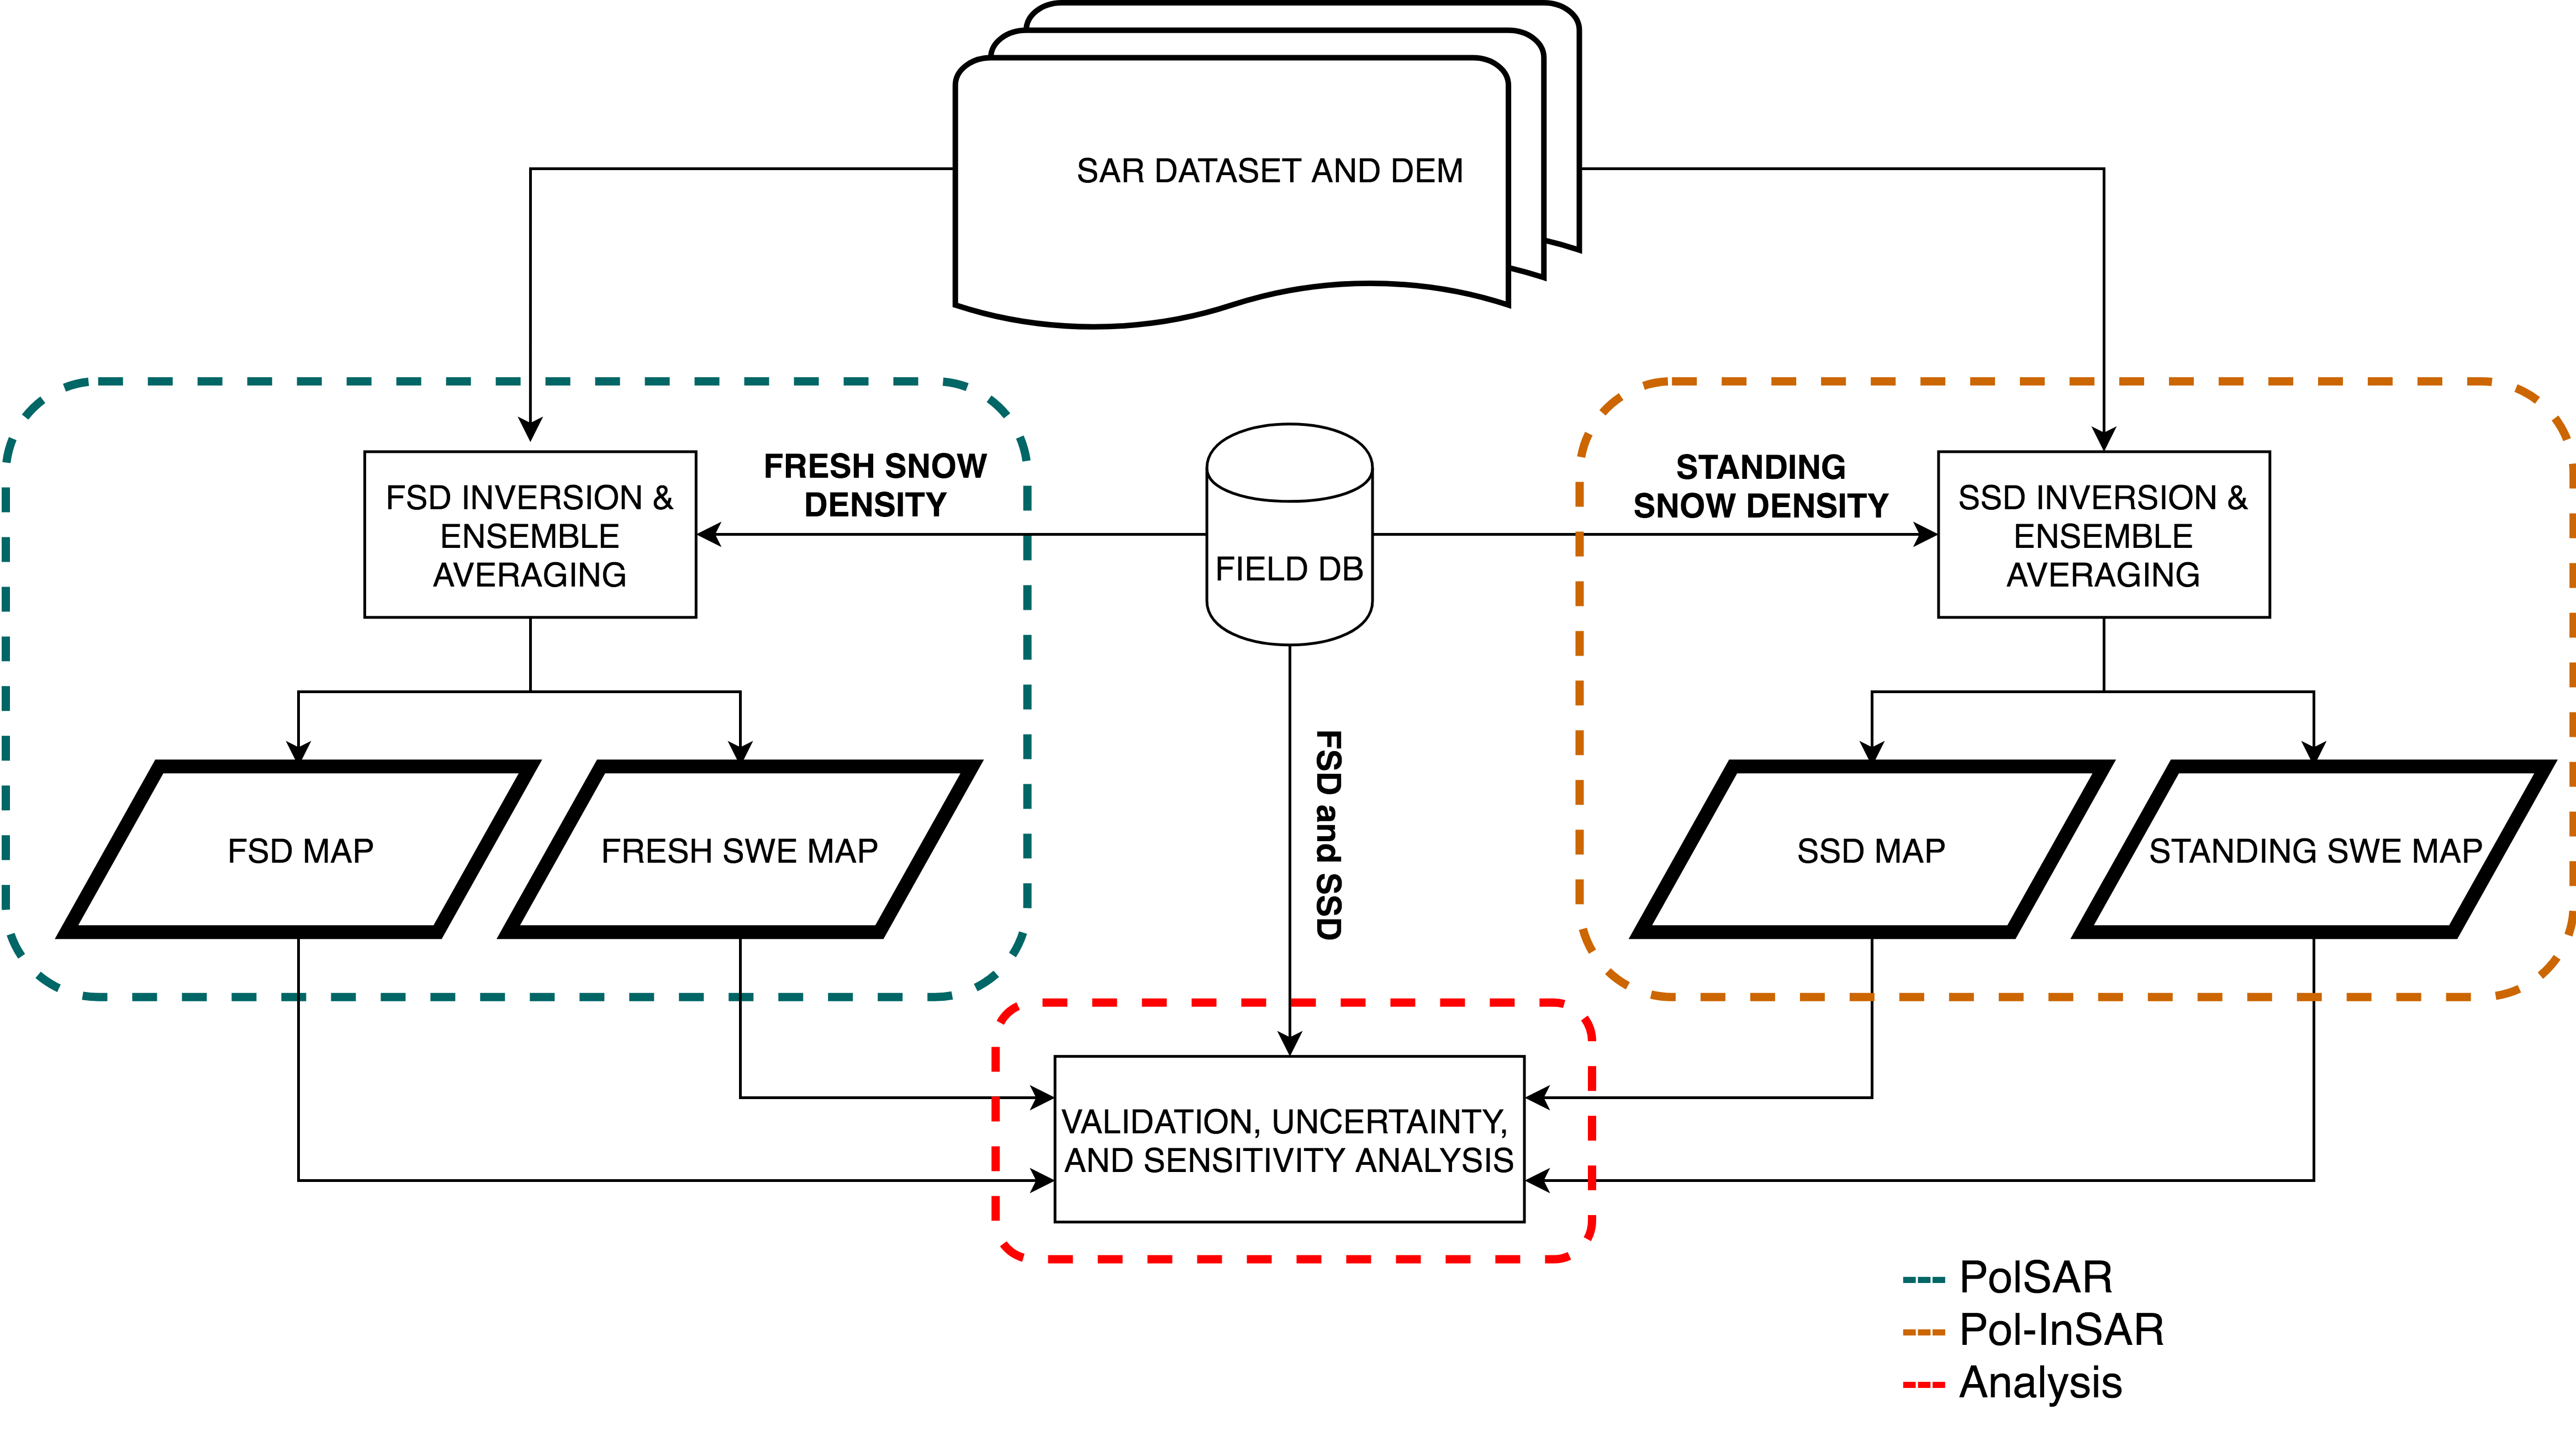
\includegraphics[width=\textwidth]{Figures/Methods/Overview_Method.png}
    \caption{Overview of the main processing blocks.}
    \label{fig:method_overview}
\end{figure}

\subsection{Data Preprocessing}
\label{ssec:pre}

Since the SAR dataset is already coregistered, separate coregistration step has not been performed. In case of the FSD estimation model, the geocoded or terrain-corrected data (3 m spatial resolution) consists of the HH and VV scenes along with the local incidence angle (LIA) computed from the ALOS PALSAR DEM. As for the Pol-InSAR scenario, all the SAR channels, i.e., HH, HV, VH and VV along with the LIA are present in the geocoded data. It should be noted that, for the Pol-InSAR, processing both the master, TDX (master) and TSX (slave) images are required to generate the interferogram. However, the FSD estimation model can be used using any one of these images, though the average of the TDX and TSX CPDs can potentially improve the signal-to-noise ratio (SNR) \citep{Leinss2014}.

\subsection{CPD based Fresh Snow Depth Estimation}
\label{ssec:fsd}
\subsubsection{CPD Computation}

The FSD is estimated using the CPD method developed by \cite{Leinss2014}. At first, $\phi_{CPD}$ for the TDX data ($\phi_{CPD,TDX}$) acquired on January 8, 2016, is computed using Eq. \eqref{seq:a} and then an ensemble averaging operation is applied over a 21$\times$21 window \citep{Majumdar2019}. Similarly, $\phi_{CPD}$ for the TSX data ($\phi_{CPD,TSX}$) is calculated following which the average CPD, $\overline{\phi_{CPD}}$ is obtained using Eq. \eqref{seq:b}. Here, $\Im$ and $\Re$ denote the imaginary and real parts of the complex scattering matrices $S_{VV}$ and $S_{HH}$ respectively.

\begin{subequations}
    \centering
    \label{eq:1}
    \begin{equation}
        \phi_{CPD} = \phi_{VV} - \phi_{HH} = \left\langle\underbrace{\tan^{-1}\left(\frac{\Im\left(S_{VV}\right)}{\Re\left(S_{VV}\right)}\right)}_{\phi_{VV}} - \underbrace{\tan^{-1}\left(\frac{\Im\left(S_{HH}\right)}{\Re\left(S_{HH}\right)}\right)}_{\phi_{HH}}\right\rangle
        \label{seq:a}
    \end{equation}
    
    \begin{equation}
        \overline{\phi_{CPD}} = \frac{\phi_{CPD,TDX} + \phi_{CPD,TSX}}{2}
        \label{seq:b}
    \end{equation}
\end{subequations}

 $\phi_{CPD}$ can be alternatively defined as the phase angle of the complex copolar coherence, $\widetilde{\gamma_c}$ (since $\gamma$ is the standard notation for coherence amplitude, $\widetilde{\gamma}$ is used for the complex coherence), defined in Eq. \eqref{eq:2}. In this case, the copolar coherence amplitude ($\gamma_c = \lvert\widetilde{\gamma_c}\rvert$) is a measure of the radar backscattering mechanism where low values close to zero (ideally $\gamma_c =$ 0) indicate the presence of volume scattering and high values (ideally $\gamma_c =$ 1) represent surface scattering \citep{Lee2009, Leinss2014, Singh2014}. It should be noted that only the CPD computed from side-looking radar systems is able to describe a target having dielelectrically anisotropic microstructure as in the case of snow \citep{Leinss2014}. 

\begin{equation}
        \widetilde{\gamma_c} = \frac{\left\langle S_{VV}S_{HH}^*\right\rangle}{\sqrt{\left\langle S_{VV}S_{VV}^*\right\rangle\left\langle S_{HH}S_{HH}^*\right\rangle}} = \gamma_ce^{j\phi_{CPD}}, \gamma_c \in [0, 1]
        \label{eq:2}
\end{equation}

\subsubsection{Calculating the Depolarisation Factors}

In order to model this snow anisotropy, an ice particle needs to be associated with a specific shape. It has been observed that fresh snow and old snow exhibit horizontally aligned (oblate) and vertically aligned (prolate) spheroidal structures respectively \citep{Leinss2014}. Moreover, a shape parameter, known as the depolarisation factor, also has to be considered in this context \citep{Leinss2014, Sihvola1999}. In principle, a single spheroidal particle is characterised by three dipoles corresponding to the three orthogonal axes ($a_x$ , $a_y$ , and $a_z$) represented using a 3D ($x$, $y$, $z$) Cartesian coordinate system. This is depicted in Figure \ref{fig:prolate}, where the prolate shaped ice grain is linked with the radar reference frame ($h$, $k$, $v$) following the radar backscattering alignment (BSA) convention, $k$ being the propagation vector, $h$ and $v$
are the wave components of the horizontal and vertical polarisations respectively. Also, $\theta$ is the mean incidence angle with respect to the surface normal \citep{Leinss2014, Parrella2013}. 

\begin{figure}[htb]
    \centering
    
\includegraphics[width=\textwidth]{Figures/Prolate_New.png}
    \caption{Orientation of a single prolate ice particle linked with the radar reference frame. Adapted from \cite{Leinss2014}.}
    \label{fig:prolate}
\end{figure}

So, by fixing a particle shape, the three depolarisation factors, $N_i$ ($\forall i \in {x, y, z}$), can be obtained by
solving the surface integral ($s$ is the ellipsoidal surface) as shown in Eq. \eqref{eq:3}.

\begin{equation}
	N_i =\frac{a_xa_ya_z}{2}\int_0^\infty\frac{\mathrm{d}s}{(s+a_i^2)\sqrt{(s+a_x^2)(s+a_y^2)(s+a_z^2)}}
	\label{eq:3}
\end{equation}
\begin{center}\text{where, $N_x + N_y + N_z = 1$}\end{center}

For a perfectly spherical shape, all three depolarisation factors are equal to 1/3. The two other special
cases include disk (1, 0, 0) and needle (0, 1/2, 1/2). In cases of prolate and oblate spheroids, the closed
form expressions are already available as shown in Eq. \eqref{eq:4} \citep{Sihvola1999}. Here, the shape is dependent
on the axial ratio ($a_x/a_z$) which is used for calculating the prolate eccentricity, $e_1 = \sqrt{1 - (a_x/a_z)^2}$ , and
oblate eccentricity, $e_2 = \sqrt{(a_x/a_z)^2 - 1}$ respectively, i.e., for prolate, $a_x/a_z < 1$, whereas for oblate, it
is the reverse. However, for general ellipsoids having different axes, the above surface integration needs to
be explicitly solved.

\begin{equation}
	N_z = \begin{cases} 
          \frac{1 - e_1^2}{2e_1^3}\left(\ln{\frac{1 + e_1}{1 - e_1} - 2e_1}\right) &, a_z > a_x = a_y \\
          \frac{1 + e_2^2}{e_2^3}\left(e_2 - \tan^{-1}e_2\right) &, a_z < a_x = a_y
       \end{cases}
	\label{eq:4}
\end{equation}

\subsubsection{Computing the Snow Refractive Indices}

Evidently, the Maxwell-Garnett theory related to electromagnetic mixing models can be applied to a medium (here snow) consisting of both air and ice which are having relative permittivities, $\epsilon_{air}$ and $\epsilon_{ice}$ respectively. Therefore, the effective permittivity of this mixed medium, $\epsilon_{eff, i}$, is anisotropic and given by Eq. \eqref{eq:5} \citep{Leinss2014, Sihvola1999}. Here, the particle volume fraction ($f_{vol}$) is dependent on the fresh snow density ($\rho_f$)and ice density ($\rho_{ice}$). 

\begin{equation}
	\epsilon_{eff, i} = \epsilon_{air}\left[1 + f_{vol}\frac{\epsilon_{ice} - \epsilon_{air}}{\epsilon_{air} + \left(1 - f_{vol}\right)N_i\left(\epsilon_{ice} - \epsilon_{air}\right)}\right]
	\label{eq:5}
\end{equation}
\begin{center}where, $f_{vol} = \rho_f / {\rho_{ice}}, \rho_{ice} = 0.917 \text{ g/cm\textsuperscript{3}, and } i \in {x, y, z}$\end{center}

Furthermore, the refractive indices of this birefringent (or birefractive) medium, $n_H$ and $n_V$ corresponding to the HH and VV polarisations respectively, are dependent on this anisotropic effective permittivity \citep{Leinss2014}. In addition, since the snow anisotropy is assumed to be oriented along the Earth’s gravitational field, $n_H$ remains constant whereas $n_V$ is dependent on the incidence angle $\theta$ as given by Eq. \eqref{seq:nh} and Eq. \eqref{seq:nv} respectively \citep{Leinss2016}. Also, the imaginary part of the effective permittivity is negligible in the case of dry snow (fresh snow is also dry), and therefore, it is not used in the model developed by \cite{Leinss2014}.

\begin{subequations}
    \centering
    \label{eq:6}
    \begin{align}
        n_H^2 &= \epsilon_{eff, x} \label{seq:nh}\\
        n_V^2 &= \epsilon_{eff, y}\cos^2\theta + \epsilon_{eff, z}\sin^2\theta \label{seq:nv} 
    \end{align}
\end{subequations}
where, $\epsilon_{eff, x}$ , $\epsilon_{eff, y}$ , and $\epsilon_{eff, z}$ represent the effective permittivities of fresh snow in $x$, $y$, and $z$ directions of a 3D Cartesian co-ordinate system \citep{Leinss2014}.

\subsubsection{FSD and FSWE Computation}

Once all these aforementioned parameters are calculated, the CPD based inversion model given by Eq. \eqref{eq:7} is applied to estimate the depth of fresh snow, denoted by $\Delta{Z_f}$ \citep{Majumdar2019, Leinss2014, Leinss2016}. In this equation, -1 is introduced as per the BSA convention which is followed for all radar systems. Here, $\lambda_0$ is the radar wavelength and $\Delta\zeta$ is the relative path length difference which is dependent on $\epsilon_{eff, i}$, $\theta$, and $\rho_f$ \citep{Leinss2016}. Moreover, the horizontally aligned microstructure of fresh snow reduces the propagation speed for the HH channel and hence, in this case, $n_H > n_V$ always holds. However, for recrystallised snow having vertically aligned structures, the reverse condition is true \citep{Leinss2016}. Also, the LIA ($\theta_l$) is used instead of the mean incidence angle ($\theta$) to consider the effect of the terrain slope.

\begin{equation}
    \centering
    \Delta{Z_f} = (-1)\frac{\lambda_0\phi_{CPD}}{4\pi\Delta{\zeta}}
    \label{eq:7}
\end{equation}
\begin{center}where, $\Delta{\zeta} = \sqrt{n^2_V - \sin^{2}\theta_l} - \sqrt{n^2_H - \sin^{2}\theta_l}, \phi_{CPD} > 0, \text{ and } n_H > n_V$\end{center}

Here, the depolarisation factors are calculated by setting the axial ratio, $a_x/a_z = 1.6$ in
Eq. \eqref{eq:4} and choosing the snow particle shape as an oblate \citep{Majumdar2019}. After this, the anisotropic
effective permittivities are computed using Eq. \eqref{eq:5}. Finally, the FSD is obtained from Eq. \eqref{eq:7} wherein an ensemble averaging filter of size 65$\times$65 is applied. The FSWE is obtained by multiplying the FSD with the fresh snow density (i.e, FSWE $ = \Delta{Z_f}\rho_f$)Also, the fresh snow density ($\rho_f = $0.07 g/cm\textsuperscript{3}) which is manually measured at Dhundi, is kept constant for the entire study area along with the copolar coherence threshold, $\tau_c = $ 0 ($\tau_c \in$ [0, 1]), i.e., no thresholding has been applied, but the provision for it is built-in to the implementation. Moreover, as per the TSX/TDX metadata, the radar wavelength, $\lambda_0 ≈ $ 3.11 cm. In this context, the adopted workflow is depicted in Figure \ref{fig:fsd_method}.

\begin{figure}[htb]
    \centering
    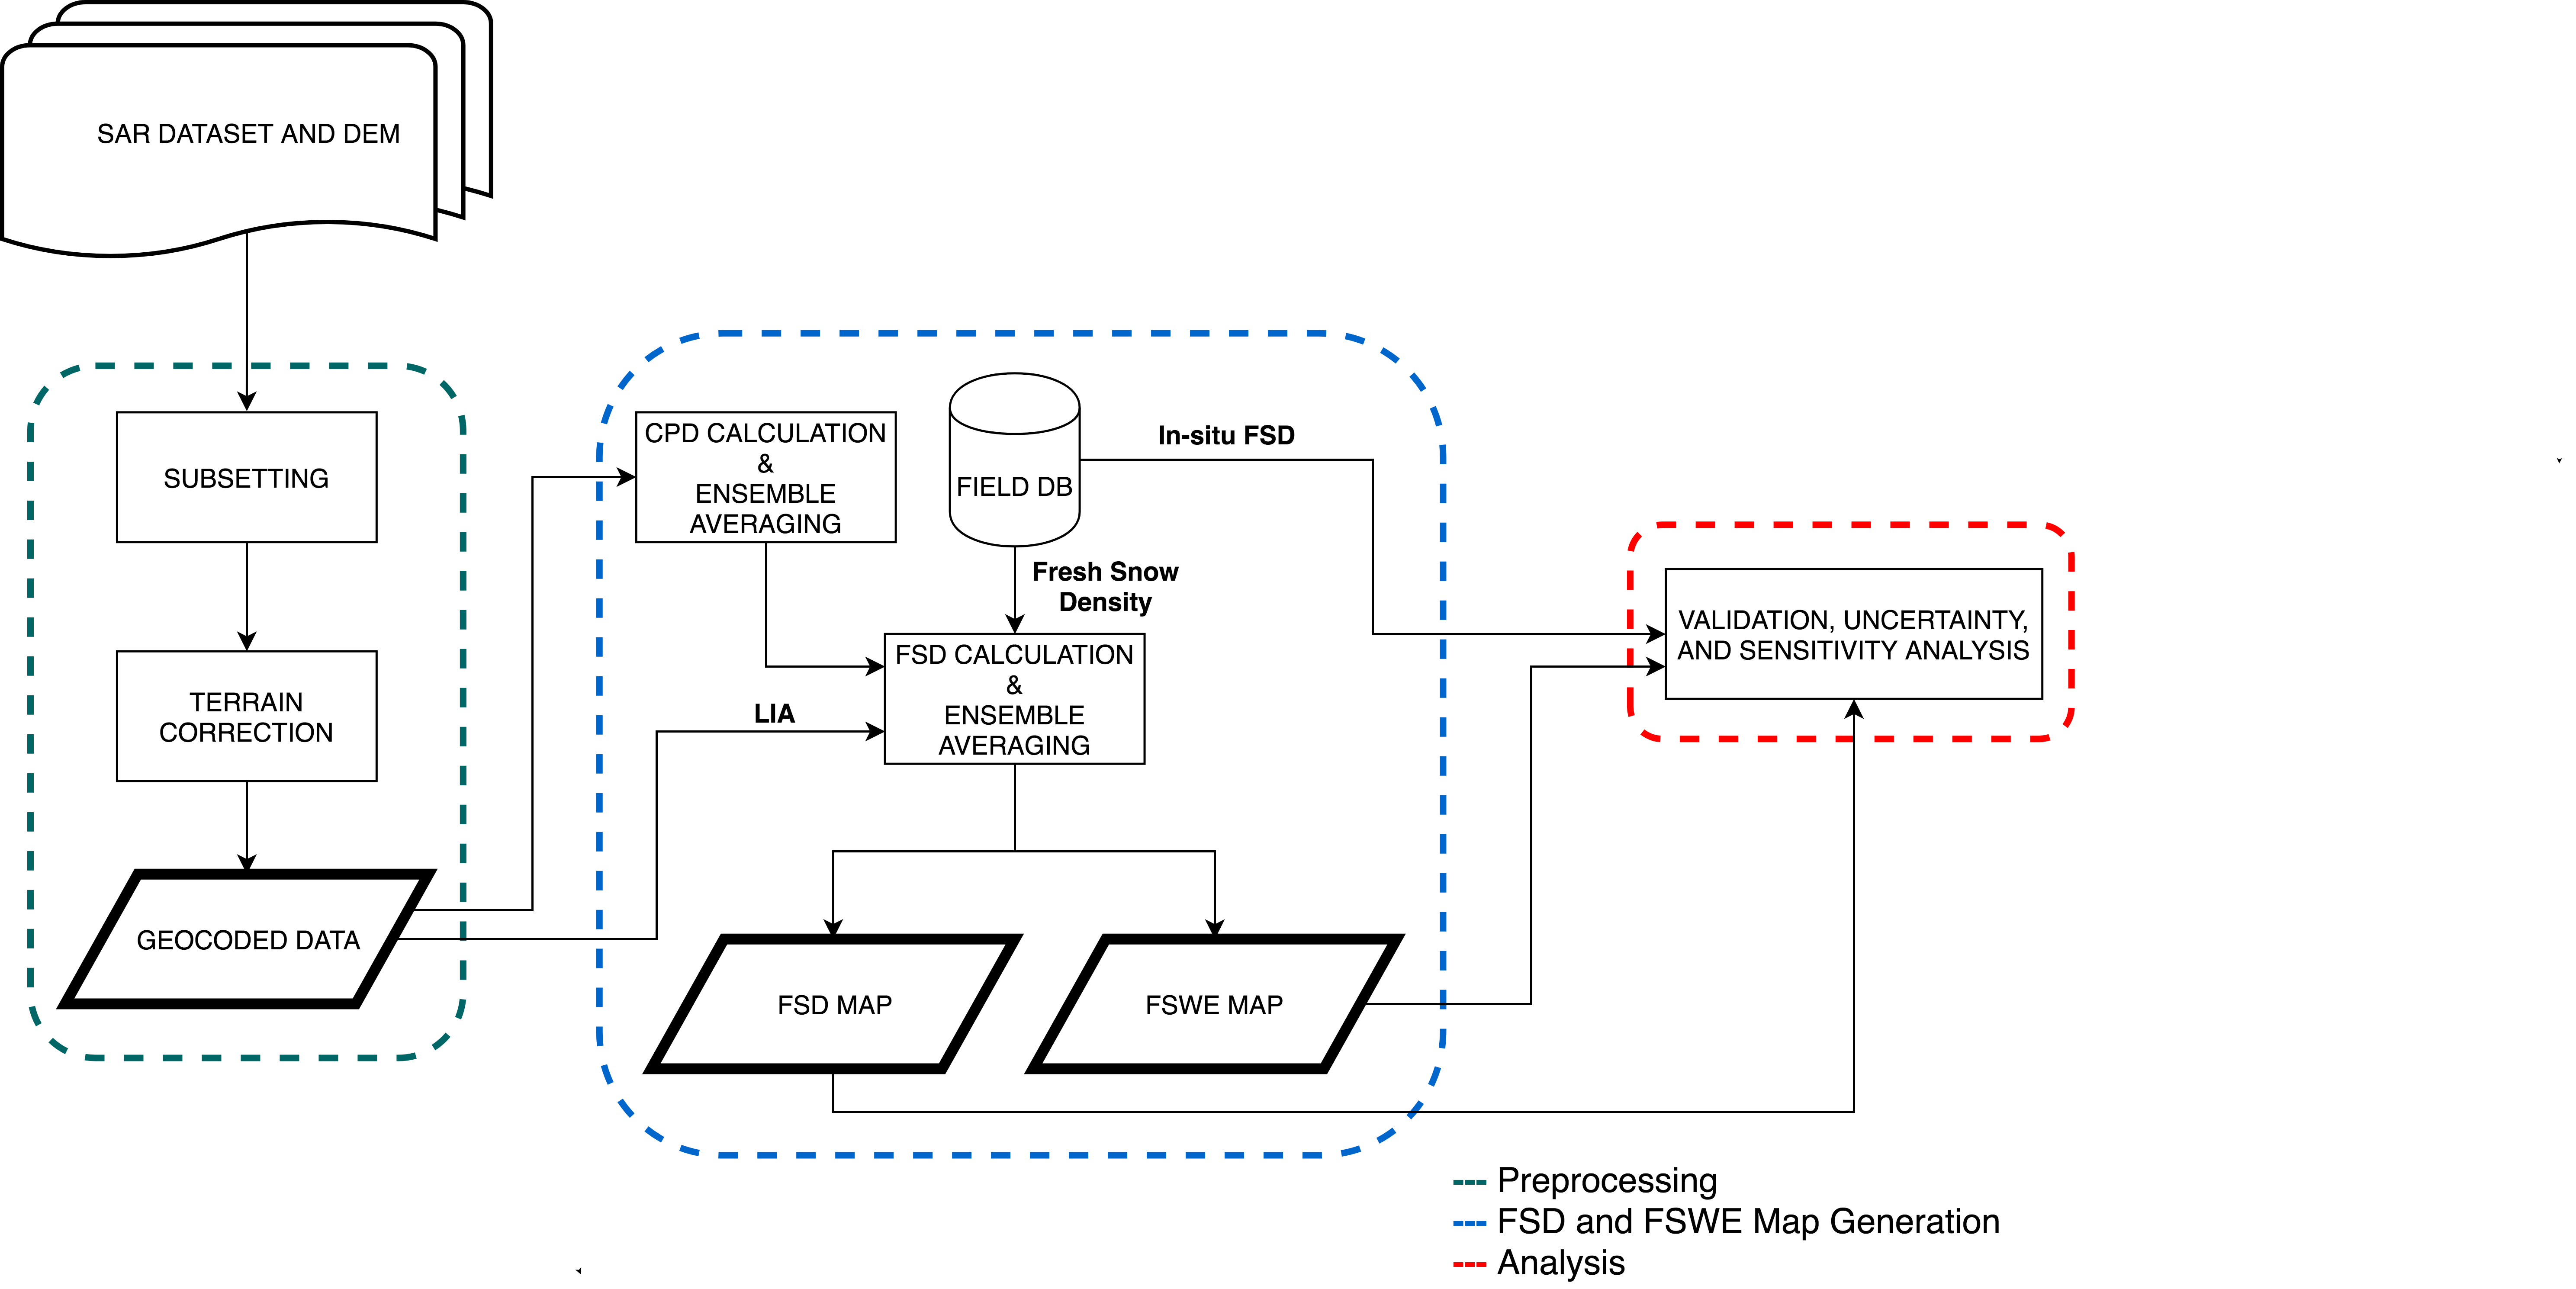
\includegraphics[width=\textwidth]{Figures/Methods/FSD_Method.png}
    \caption{FSD and FSWE estimation workflow using PolSAR CPD.}
    \label{fig:fsd_method}
\end{figure}

\subsection{Pol-InSAR based Standing Snow Depth Estimation}
\label{ssec:ssd}
\subsection{Validation, Uncertainty Assessment, and Sensitivity Analysis}
\label{ssec:vus}
\subsubsection{Validation Process}
\label{sssec:val}
\subsubsection{Uncertainty Assessment}
\label{sssec:ua}
\subsubsection{Sensitivity Analysis}
\label{sssec:sa}

\section{Results and Discussion}
\label{sec:res}
\section{Conclusion}
\label{sec:conc}

\section*{References}

\bibliography{refs}

\end{document}